\documentclass[10pt, landscape, a4paper]{article}
\usepackage{geometry}[landscape]
\usepackage{multicol}
\usepackage{graphicx}
\usepackage{amsmath} 
\usepackage{amssymb}
\usepackage{ccicons}
\usepackage{hyperref}
\usepackage{stmaryrd}


\usepackage[dvipsnames]{xcolor}

% Set page margins
\geometry{top=.8cm, left=.8cm, right=.8cm, bottom=.8cm}

% Set paragraph indentation
\setlength{\parindent}{0pt}

% Set path for assets
\graphicspath{{assets/}}

\setlength{\columnsep}{20pt}
\raggedcolumns

% _____ CUSTOM COMMANDS __________________________________________
\newcommand{\E}[0]{\mathbb{E}}
\newcommand{\R}[0]{\mathbb{R}}

\newcommand{\sgn}[0]{\text{sgn}}

\newcommand{\argmin}[1]{\underset{#1}{\text{argmin}}}
\newcommand{\argmax}[1]{\underset{#1}{\text{argmax}}}

\begin{document}
\begin{multicols*}{3}

% _____ CONTENT __________________________________________________

% main heading
\begin{center}
	\Large{\textbf{Rigorous Software Engineering}} \\
    \small{by dcamenisch}
\end{center}

\section{Introduction}

This document is a summary of the 2023 edition of the lecture \textit{Rigorous Software Engineering} at ETH Zurich. I do not guarantee correctness or completeness, nor is this document endorsed by the lecturers. If you spot any mistakes or find other improvements, feel free to open a pull request at \url{https://github.com/dcamenisch/rse-summary}. This work is published as CC BY-NC-SA.
\begin{center}
	\ccbyncsa
\end{center}
\section{Documentation}

Source code alone is not enough to document software engineering projects. Developers need additional information that is difficult to extract from source code, such as possible results of a method, possible side effects of methods, and consistency conditions of data structures. Therefore documentation is key to ensure that software is reliable and maintainable over time.

\subsection{What to document}

There are two stakeholders, clients and implementors. For clients it is important to document the interface, how to use the code. For stakeholders it is important to document how the code works. For interfaces document the methods and constructors that clients can use to interact with the software, as well as any preconditions and postconditions that must be met. When documenting the implementation for implementors include the algorithms and data structures used in the software, as well as any invariants and assertions that must be maintained.

\subsection{How to document}

Documentation does not only consist of comments. Using type annotations, modifiers, assertions and effect systems can also be considered documentation. Still, comments are a large part of good documentation. They provide simple, flexible way of documenting interfaces and implementations. A good documentation using comments can look as follows:

\begin{center}
	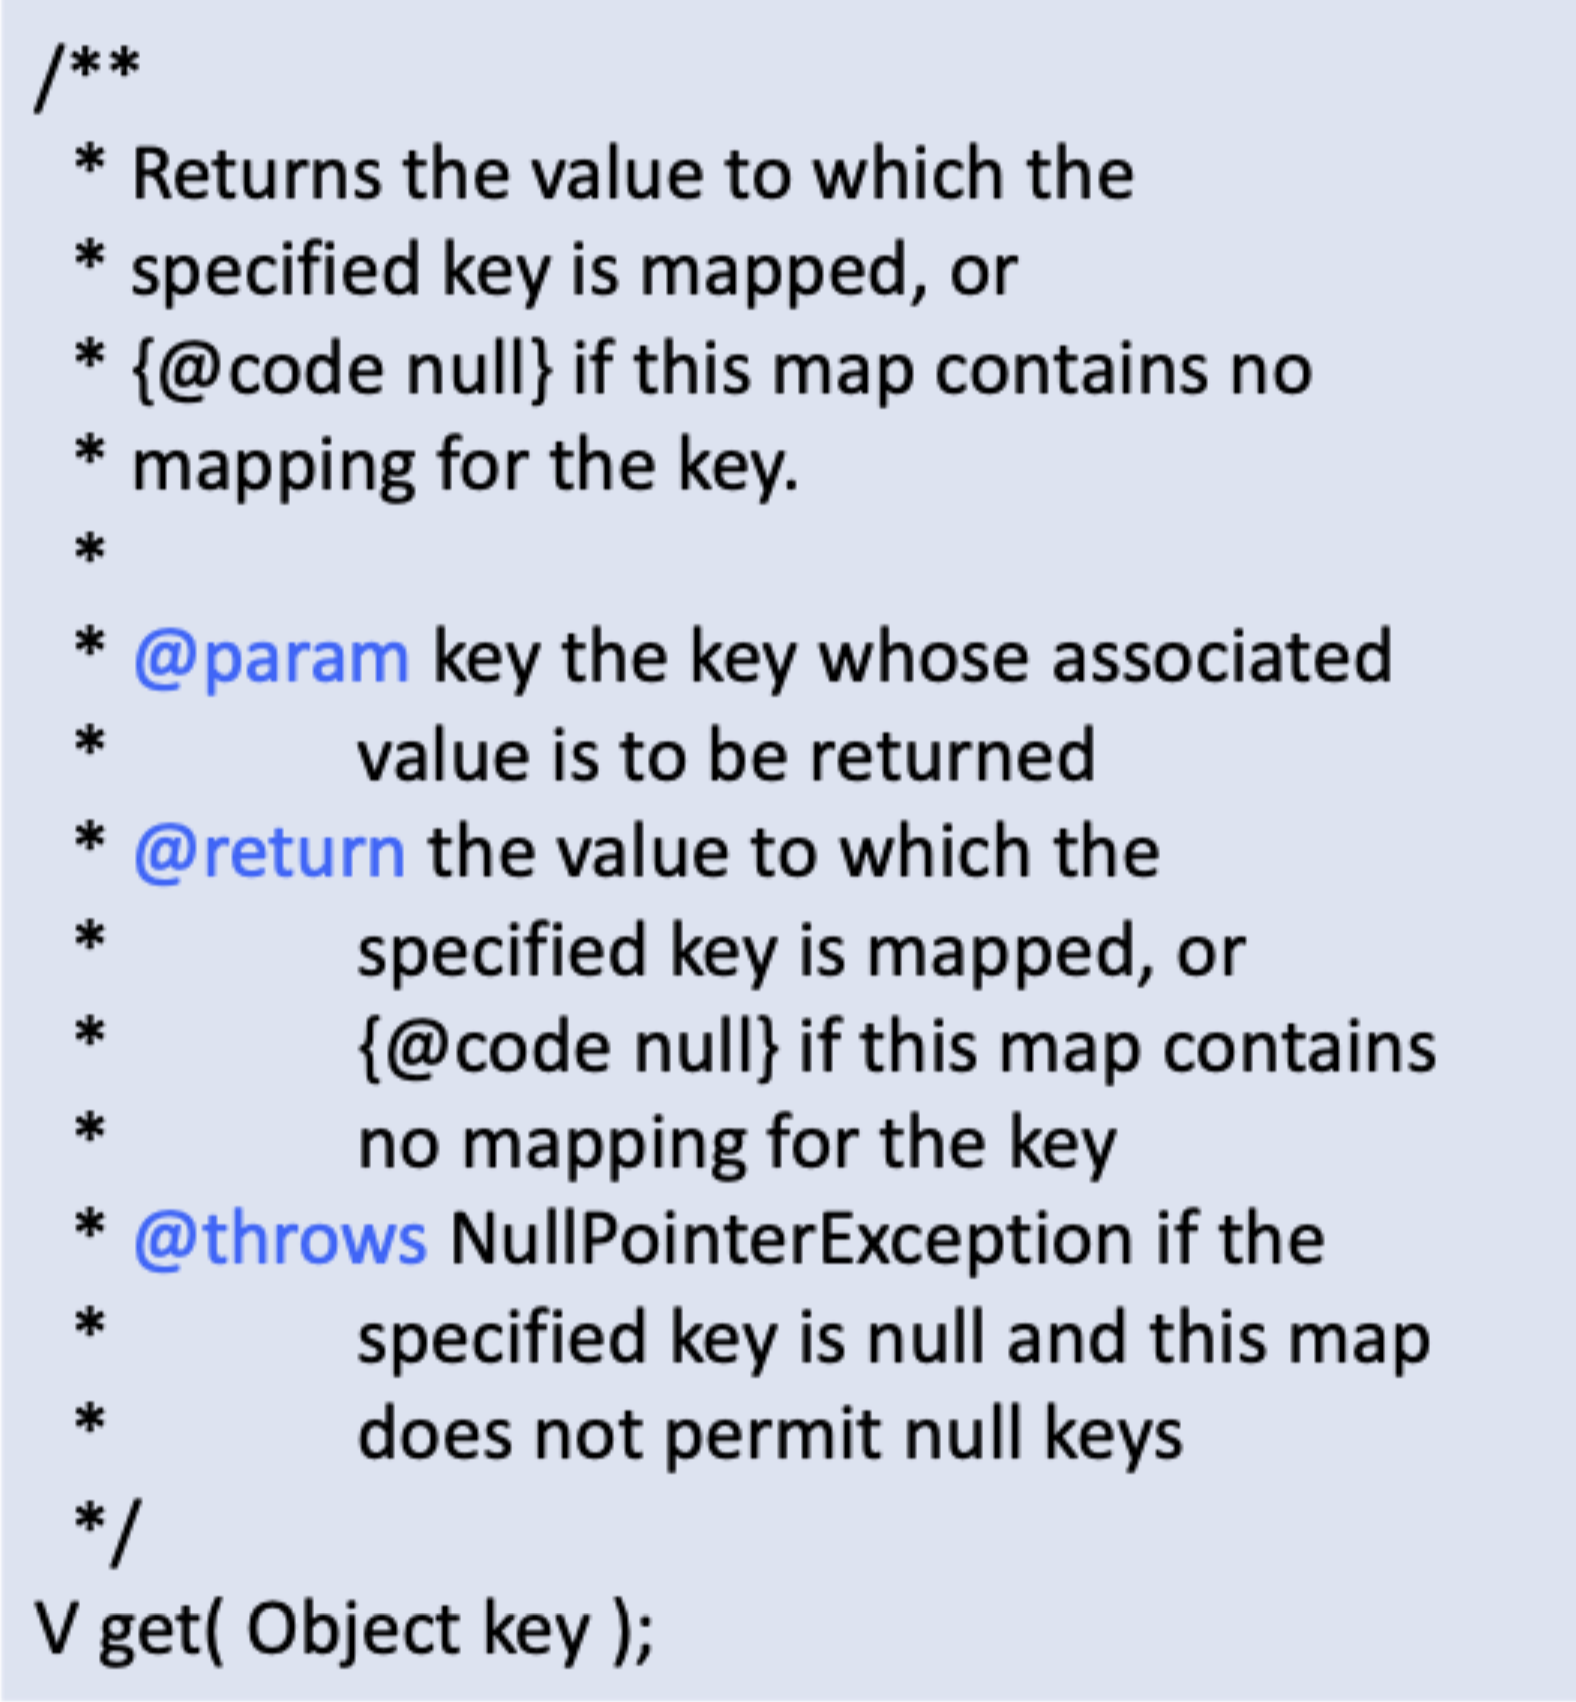
\includegraphics[width=0.5\columnwidth]{assets/comment}
\end{center}

Using diagrams and examples to illustrate complex concepts can help to make the documentation easier to understand. Using consistent formatting and naming conventions can further improve it. Finally, reviewing and updating the documentation regularly to ensure that it remains accurate and up-to-date.
\section{Modularity}

The idea of modularity is to partition the overall development effort, support independent testing and analysis of components, decouple parts so they can be modified individually and dividing a large system in mind-sized chunks.

\subsection{Coupling}

\textbf{Coupling} measures interdependence between different modules. A thigh / high coupling means that modules cannot be developed, tested, changed, understood or reused in isolation. Therefore we want low coupling for correct and maintainable software.

\subsubsection{Data Coupling}

Modules that expose their internal data representation become tightly coupled to their clients (\textbf{representation exposure}). It prevents modules from maintaining strong invariant and concurrency requires complex synchronization. Similarly, data representations often include sub-objects, exposing these can lead to unexpected side effects. \\

One way of preventing this is to restrict the access to data - forcing clients to access the data representation through a narrow interface. Avoid exposure to sub-objects and prevent the leaks of any references to these sub-objects. \\

Modules get couples by operating on shared data structures (e.g. compiler working on syntax tree). This can be avoided by making the data structure immutable, however changing the data representation remains a problem and having to copy it can lead to run-time and memory overhead. \\

The flyweight pattern is one example that tries to maximize sharing of immutable objects, it is for example used in Java for constant strings.

\subsubsection{Procedural Coupling}

Modules are coupled to other modules whose methods they call. Callers cannot be reused without callee modules and changing a signature in the callee requires changing the caller. \\

This can be prevented by moving code and even duplicating functionality to avoid dependency. Another solution could be to change to a event based system. Components may generate events and register for events from other components using a callback. Event generators do not know which components will be affected by their events (loss of control). \\

One common event based architecture is Model-View-Controller. The model contains the core functionality and data, the view is responsible for displaying information and the controller handles user inputs. All communication happens via events and the model and the view are decouples through the controller.

\begin{center}
	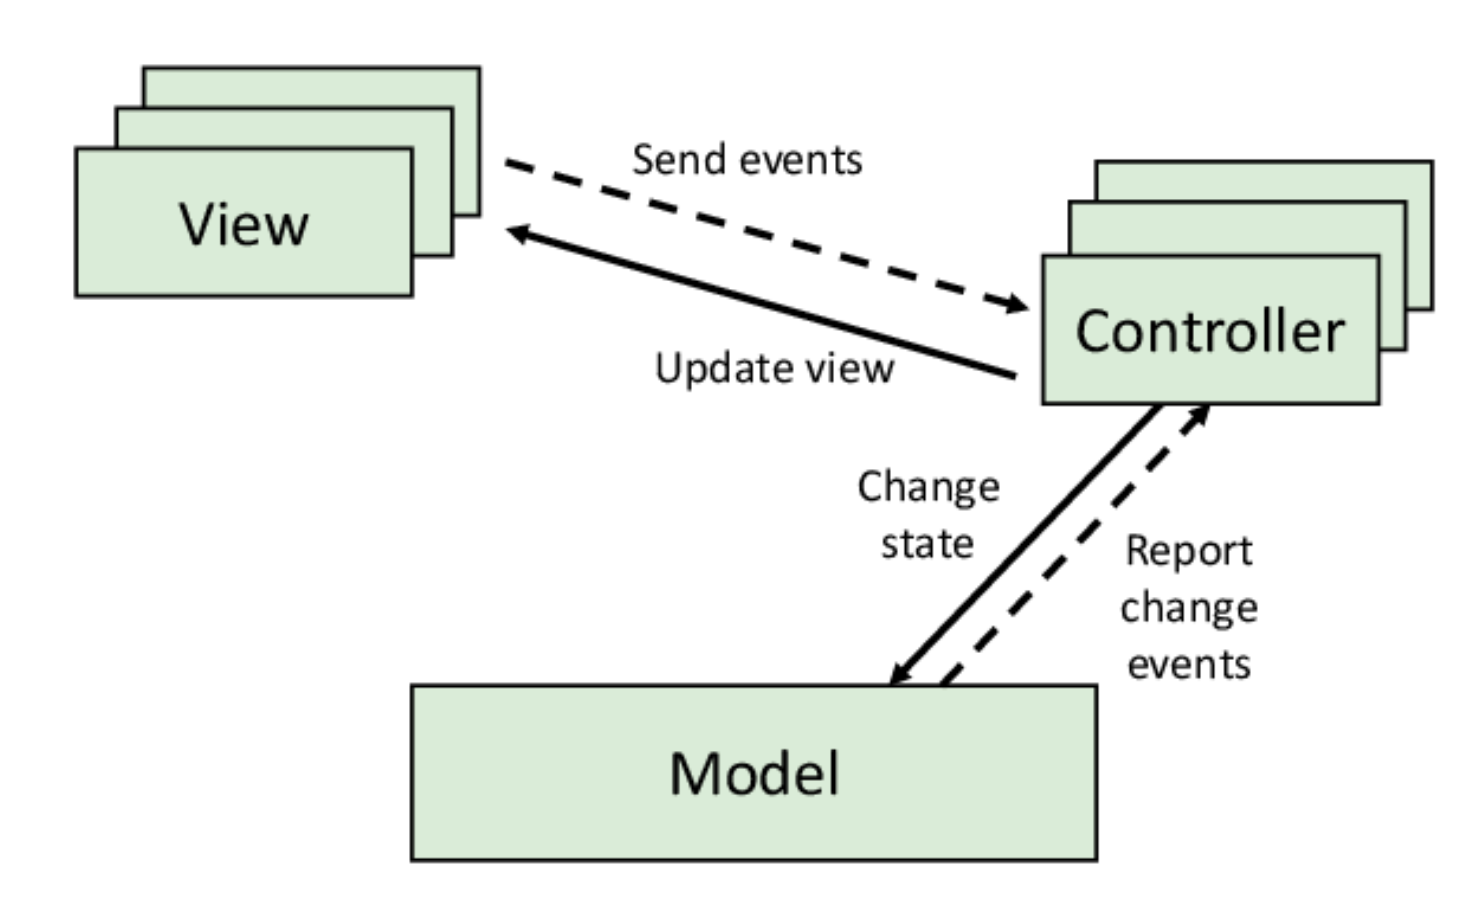
\includegraphics[width=0.5\columnwidth]{assets/mvc}
\end{center}

\subsubsection{Class Coupling}

Inheritance couples the subclass to the superclass, changes in the superclass may break the subclass. \\

To solve this, we can replace (multiple) inheritance by subtyping and delegation.

\begin{center}
	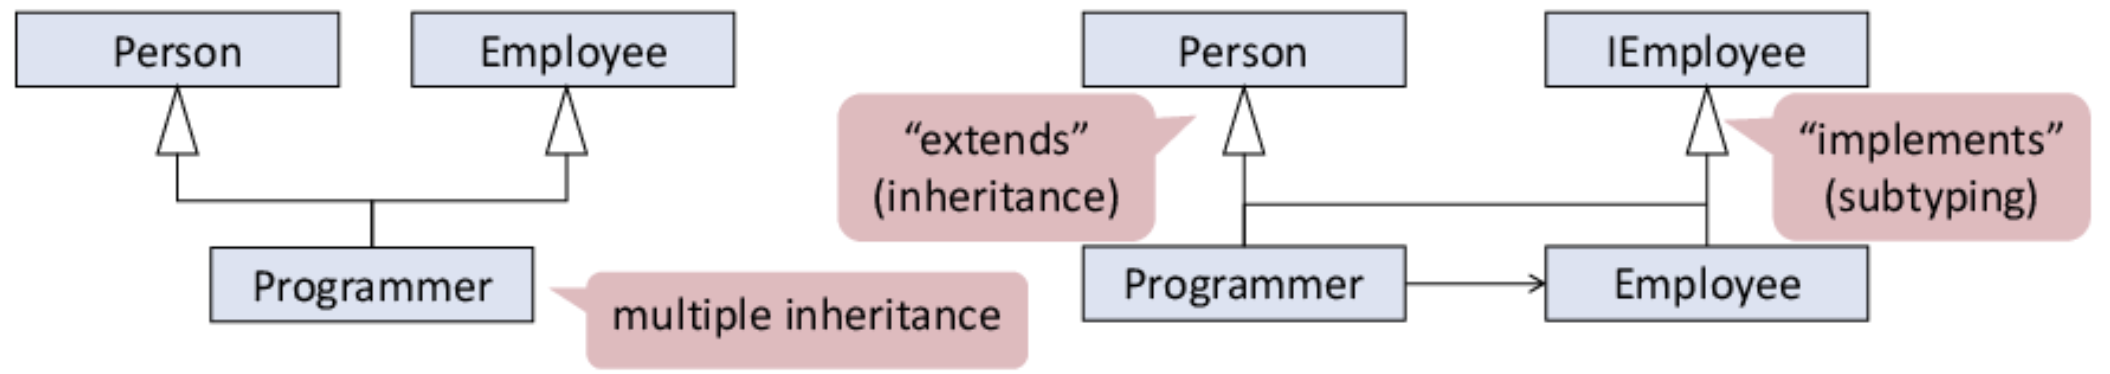
\includegraphics[width=\columnwidth]{assets/inheritance}
\end{center}

Using class names in declarations of methods, fields, and local variables couples the client to the used class. To avoid this, one can replace class names by supertypes (interfaces). Using the most general supertype that offers all required operations. \\

Lastly, allocations couples the client to the instantiated class. We fix this by using dedicated classes called abstract factories to handle allocation. 

\begin{center}
	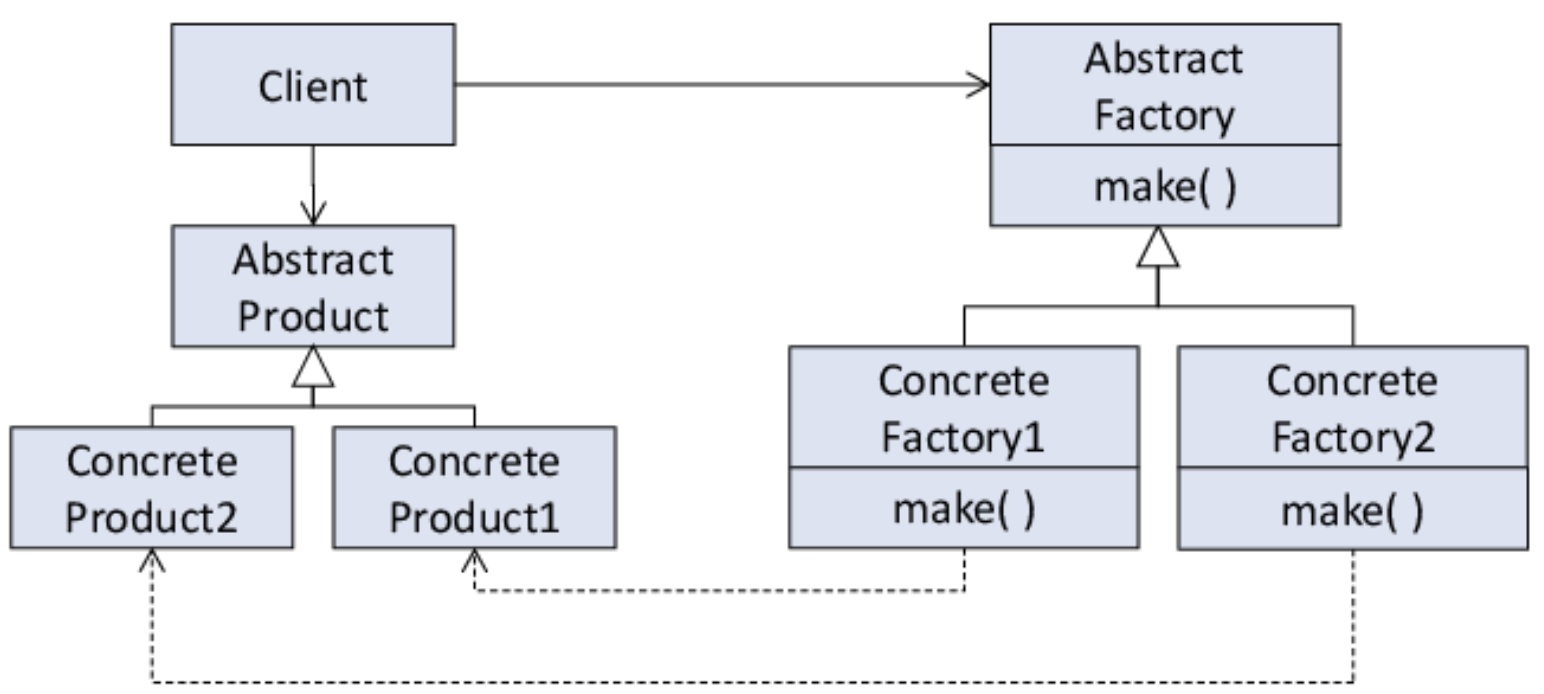
\includegraphics[width=0.7\columnwidth]{assets/factory}
\end{center}


\subsection{Adaption}

Changes often erode the structure of the system. Modules can be prepared for change by allowing clients to influence their behavior. This is done by making the module parametric in:
\begin{itemize}
	\item The value they manipulate
	\item The data structures they operate on
	\item The types they operate on
	\item The algorithms they apply
\end{itemize}

In object-oriented programs, behaviors can be specialized via overriding and dynamic method binding. Dynamic method binding is a case distinction on the dynamic type of the receiver object.
\section{Testing}

Testing is the process of executing a program with the intent of finding errors. An error is a deviation of the observed behavior from the required behavior. Testing can only show the presence of bugs and not their absence.


\subsection{Testing Stages}
\begin{center}
	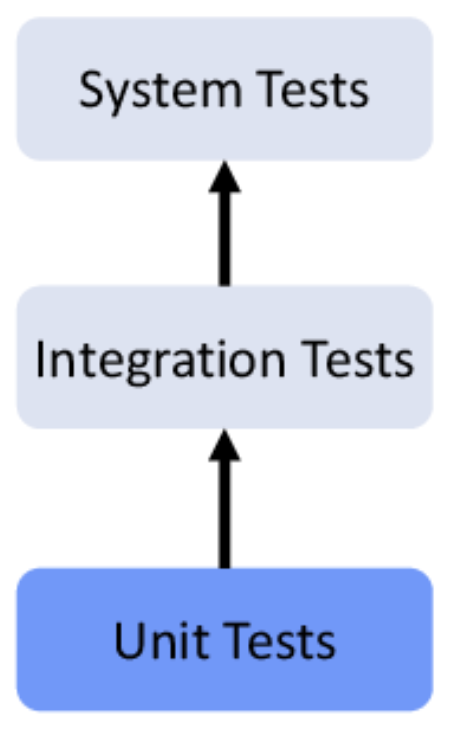
\includegraphics[width=0.2\columnwidth]{assets/testing_stages}
\end{center}

Unit testing is used to test individual subsystems (collection of classes, or a single class). To achieve a reasonable test coverage, one has to test each method with several inputs. Parameterized test methods take arguments for test data and help to decouple the test driver (logic) from the data. They also help to avoid boiler-plate code, they are most useful when test data can be generated automatically.


\subsection{Testing Strategies}

There are different strategies to testing:
\begin{itemize}
	\item Exhaustive testing - check the unit under test for all possible inputs.
	\item Random testing - select test data uniformly at random. Can be automized but it treats all inputs as equally valuable.
	\item Functional testing - use requirement knowledge to derive test cases. The goal is to cover all requirements. Does not effectively detect design and coding errors or errors in the specification.
	\item Structural testing - use design knowledge about the systems structure, algorithms, and data structures to derive test cases that exercise a large portion of the code. Focuses on covering all the code. Not well suited for system tests, due to high redundancy.
\end{itemize}

\begin{center}
	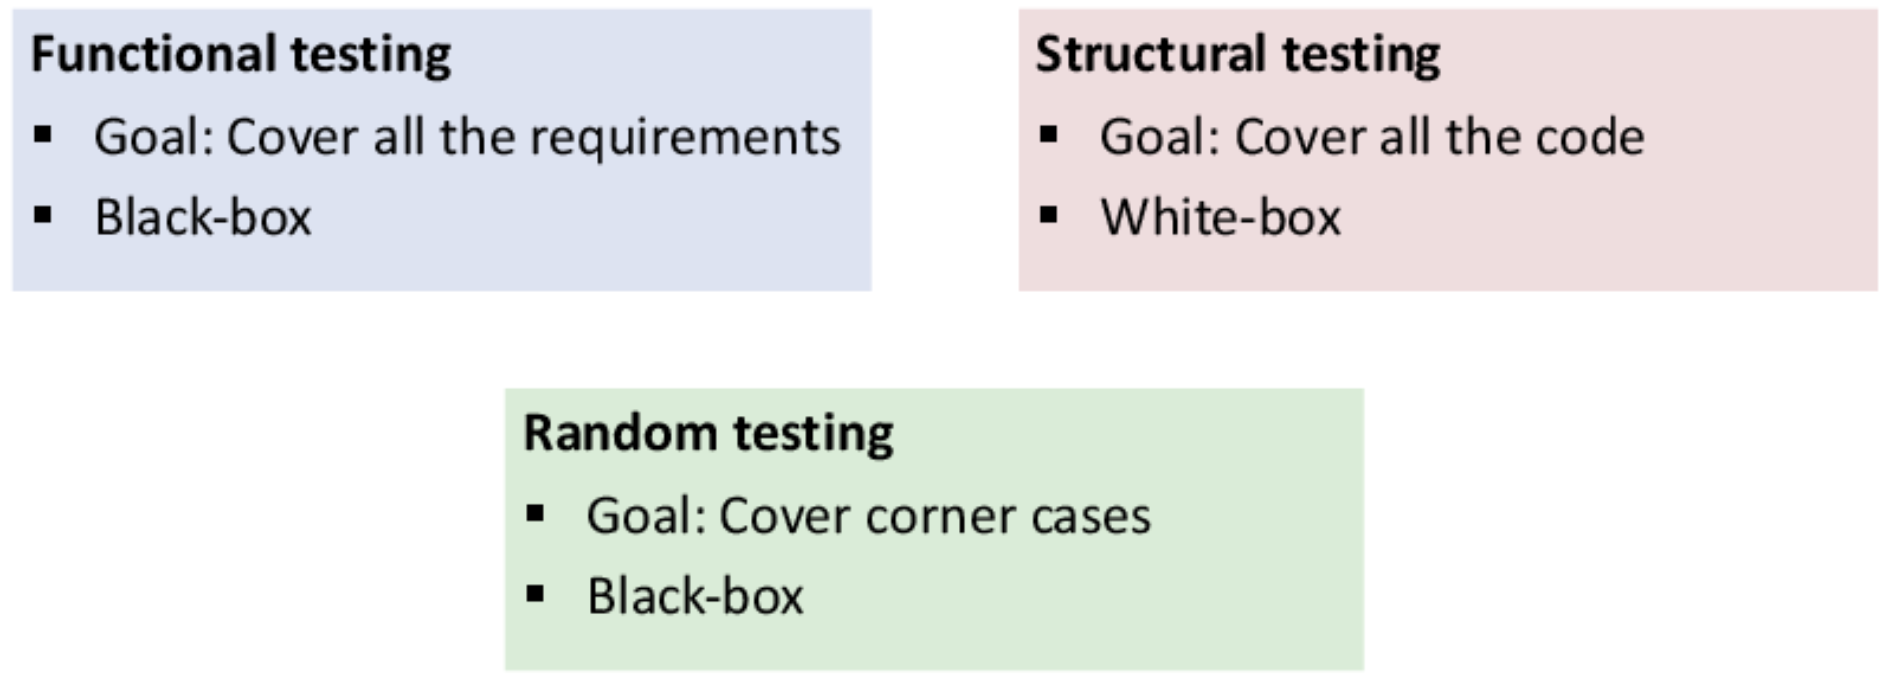
\includegraphics[width=0.9\columnwidth]{assets/testing_strategies}
\end{center}


\subsection{Functional Testing}

Functional testing black-box tests a unit against its requirements.

\subsubsection{Partition Testing}

Divide the inputs into equivalence classes and choose test cases for each equivalence class. An example for this would be to divide months into equivalence classes, based on the number of days they have.

\subsubsection{Selecting Representative Values}

After partitioning, we need to select the input values from each class. A large amount of errors tend to occur at the boundaries of the input domain (overflows, comparisons $<$ instead of $\leq$, wrong number of iterations, or missing emptiness checks). Boundary testing selects elements at the edge of each equivalence (in addition to values in the middle).

\subsubsection{Combinatorial Testing}

Combining equivalence classes and boundary testing can lead to combinatorial explosion. To reduce the amount of test cases, one can use semantic constraints, combinatorial selection or random selection. Semantic constraints use domain knowledge to remove unnecessary combinations. \\

Empirical evidence suggests that most errors do not depend on the interaction of many variables (mostly two or three variables). Therefore, it might be useful to only focus on all possible combinations of each pair of inputs.


\subsection{Structural Testing}

Detailed design and coding introduce many behaviors that are not present in the requirements, this comes down to the choice of data structures, algorithms and optimizations. Functional testing generally does not thoroughly exercise these behaviors. This is where structural testing comes in handy. \\

Basic blocks are a sequence of statements such that the code has one entry point and one exit point. Whenever the first instruction in a basic block is executed, the rest of the instructions are also executed. \\

An intraprocedural control flow graph (CFG) of a procedure $p$ is a graph $(N,E)$ where $N$ is the set of basic blocks and $E$ contains the edges from one basic block to another.

\begin{center}
	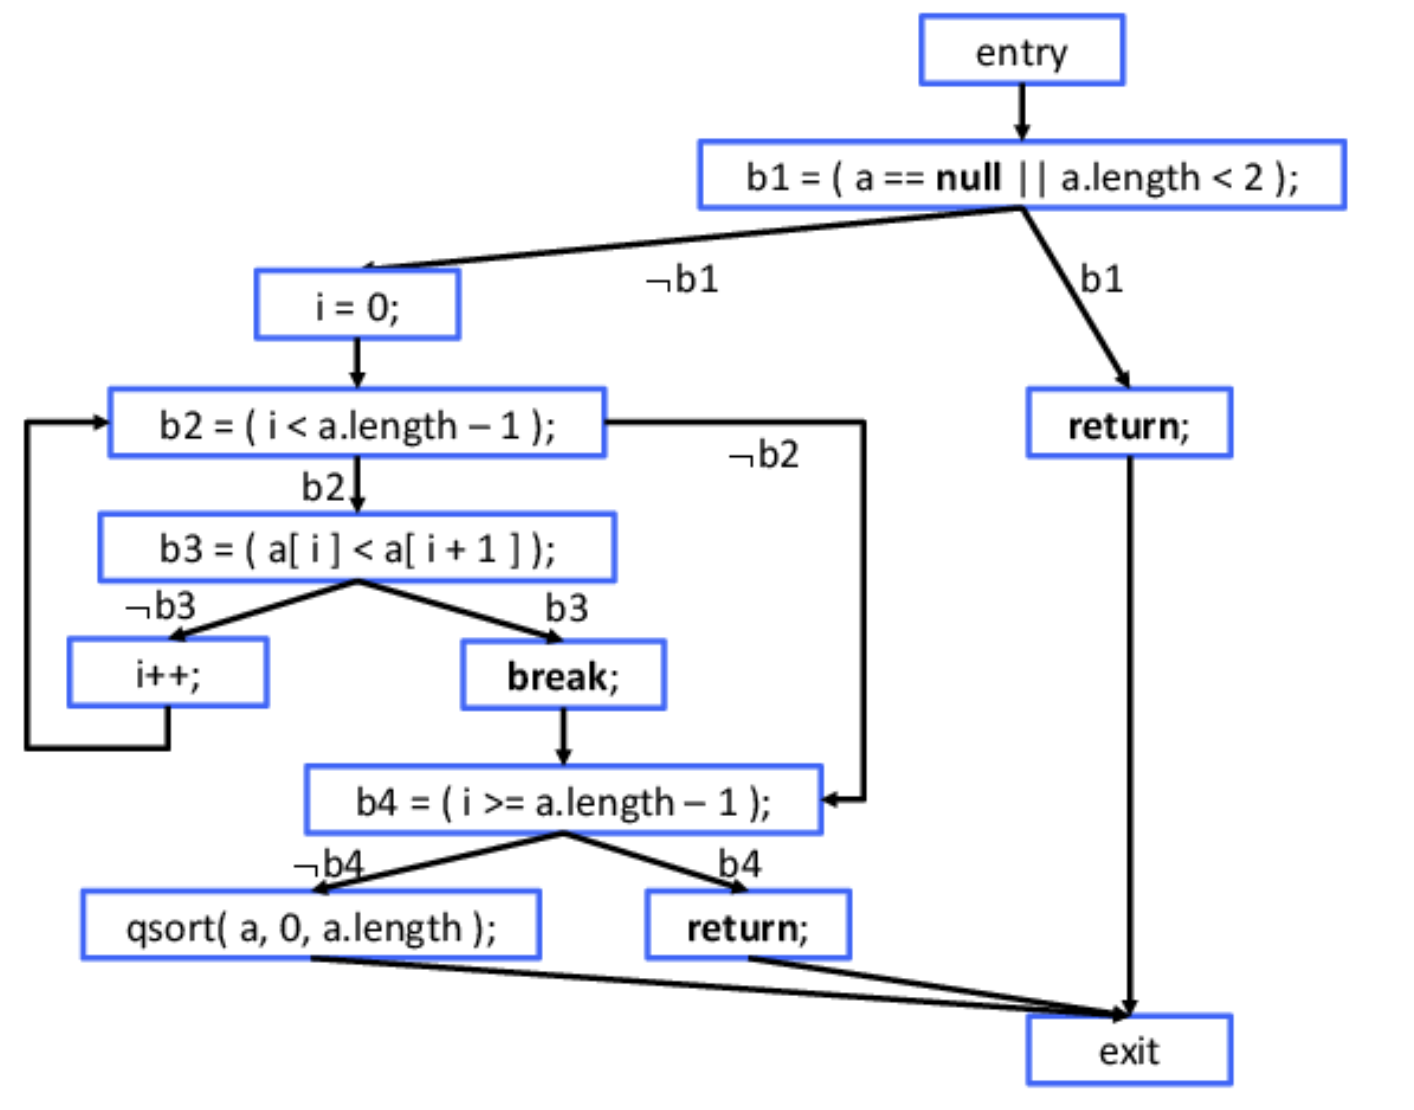
\includegraphics[width=0.8\columnwidth]{assets/cfg}
\end{center}

Statement coverage assesses the quality of a test suite by measuring how much of the CFG it executes:
$$\text{Statement Coverage } = \frac{\text{\#Executed Statements}}{\text{\#Statements}}$$

Still, 100\% statement coverage does not guarantee that we detect all the bugs, since we might not execute all edges. This is why we introduce branch coverage:
$$\text{Branch Coverage } = \frac{\text{\#Executed Branches}}{\text{\#Branches}}$$

Branch coverage leads to more thorough testing than statement coverage and is the most widely-used adequacy criterion in industry. Still, it does not guarantee that there are no bugs. Therefore, we introduce path coverage. The idea behind path coverage is to test all possible paths through the CFG:
\vspace{-5pt}
$$\text{Path Coverage } = \frac{\text{\#Executed Paths}}{\text{\#Paths}}$$

However, if for example the number of loop iterations is not known statically, an arbitrary large number of test cases is needed for complete path coverage. This leads to the final idea, loop coverage:
$$\text{Loop Coverage } = \frac{\text{\#Executed Loops w. 0, 1 and $>$1 iter.}}{\text{\#Loops} * 3}$$
\vspace{-25pt}

\section{Analysis}

The goal is to build an automatic analyzer which takes as input an arbitrary program and an arbitrary property such that the analyzer can answer if the property holds or not. But this problem is undecidable, so we have to make some sacrifices. We only want the analyzer to decided if the property holds for sure.

\begin{center}
	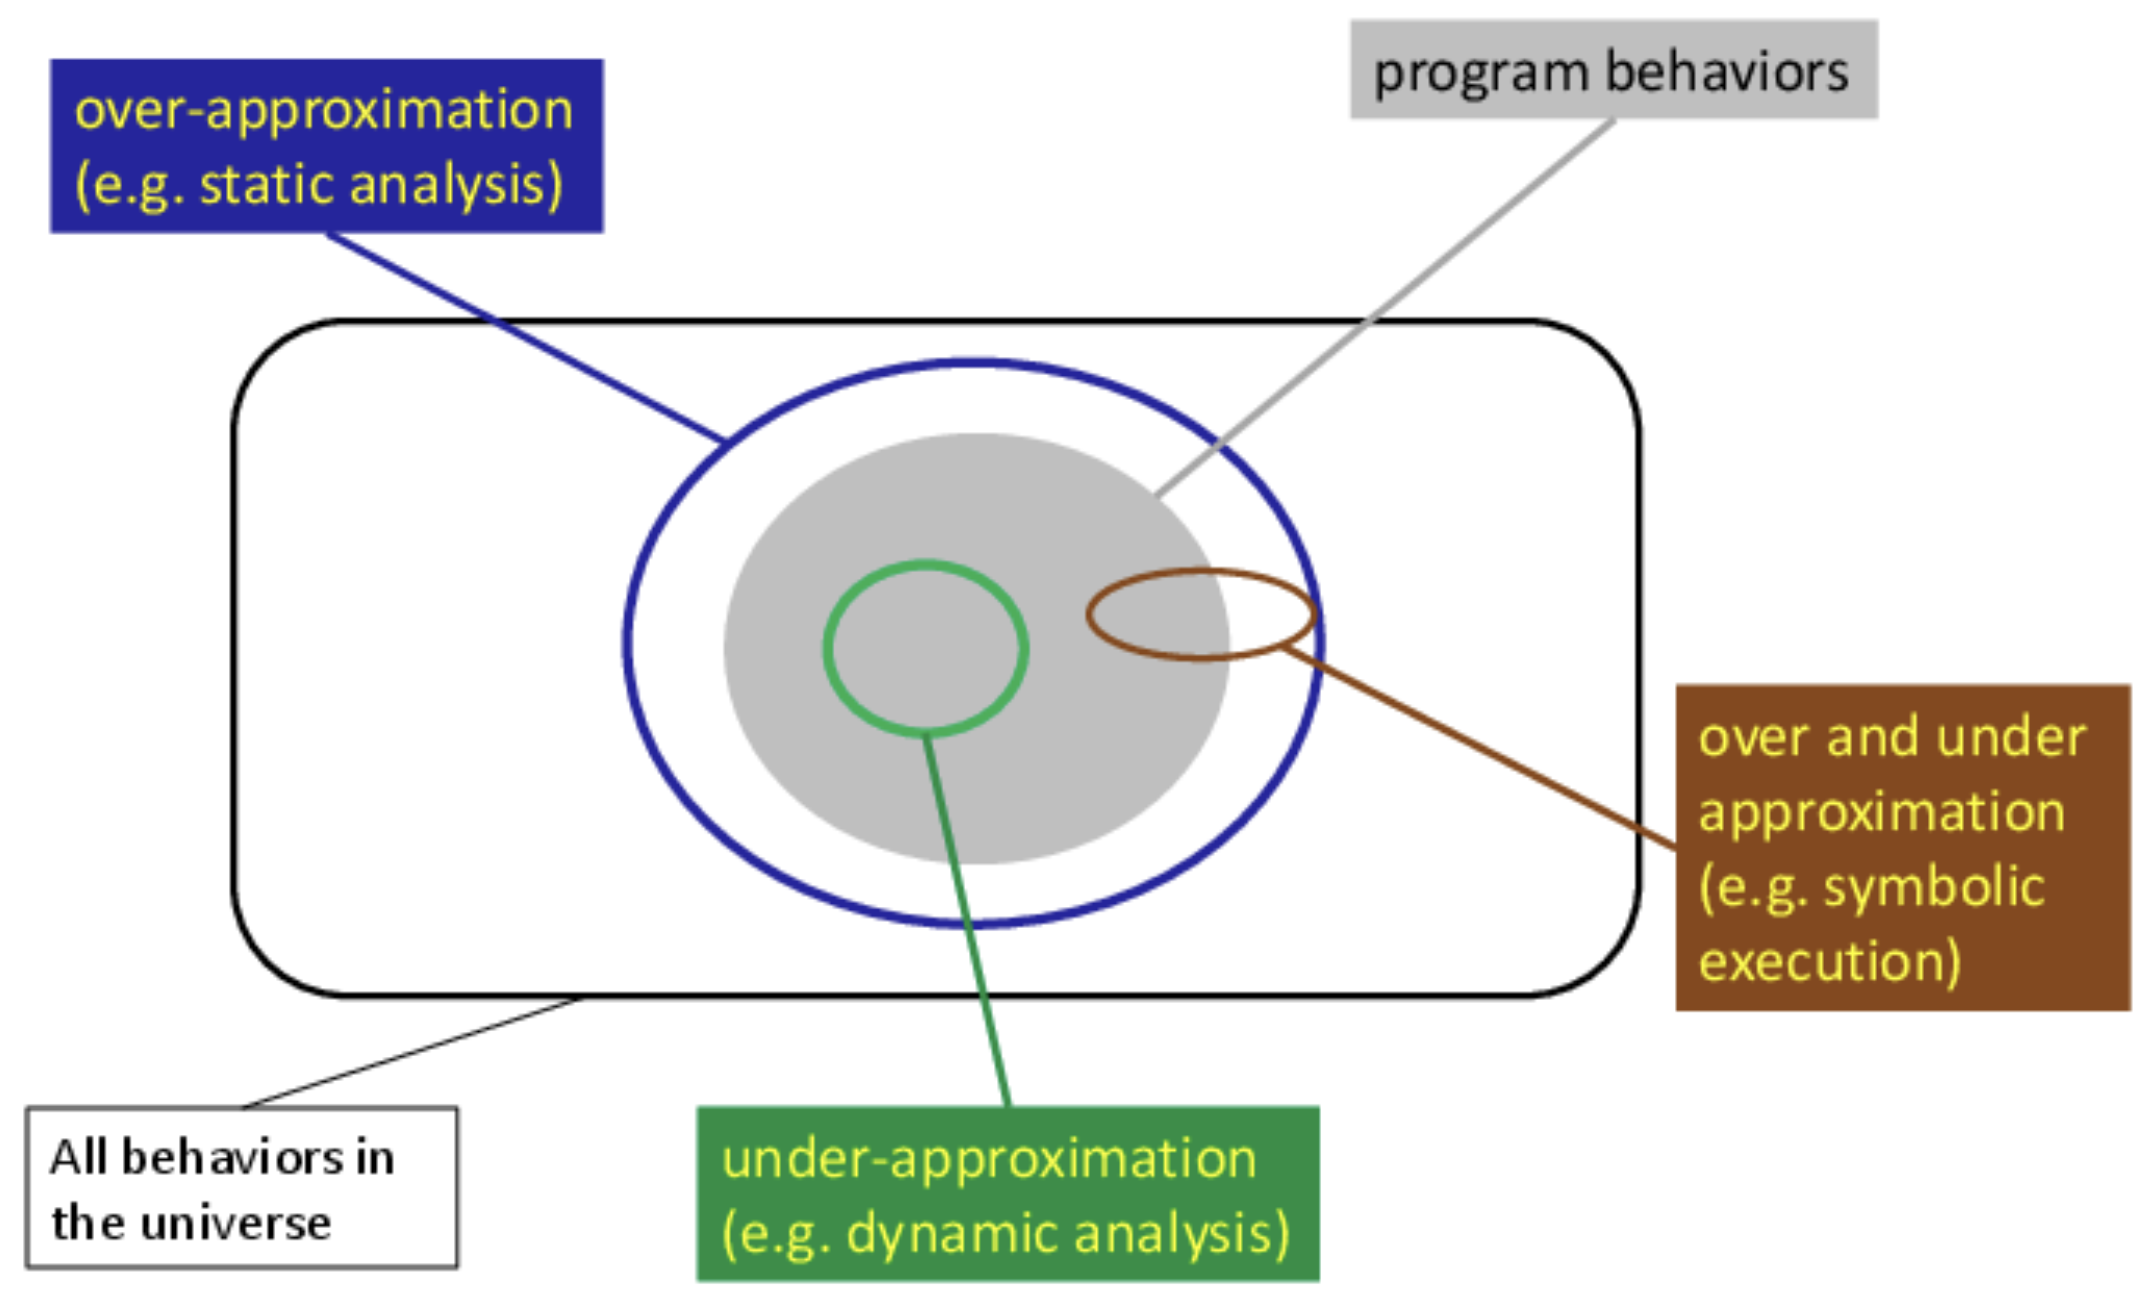
\includegraphics[width=0.8\columnwidth]{assets/program_behavior}
\end{center}

Static program analysis can run the program without giving a concrete input and does not need any manual annotations such as loop invariants.


\subsection{Abstract Interpretation}

Abstract interpretation works by:
\begin{enumerate}
	\item Select / define an abstract domain
	\item Define abstract semantics for the language w.r.t. to the domain
	\item Iterate abstract transformers over the abstract domain until a fixed point is reached
\end{enumerate}

It is important to remember that abstract transformers are defined per programming language once and for all, and not per program. A correct abstract transformer should always produce results that are a superset of what a concrete transformer would produce. In general it is easy to be sound and imprecise, being sound and precise is hard. \\

One example for this type of interpretation uses the interval domain given by:
\begin{center}
	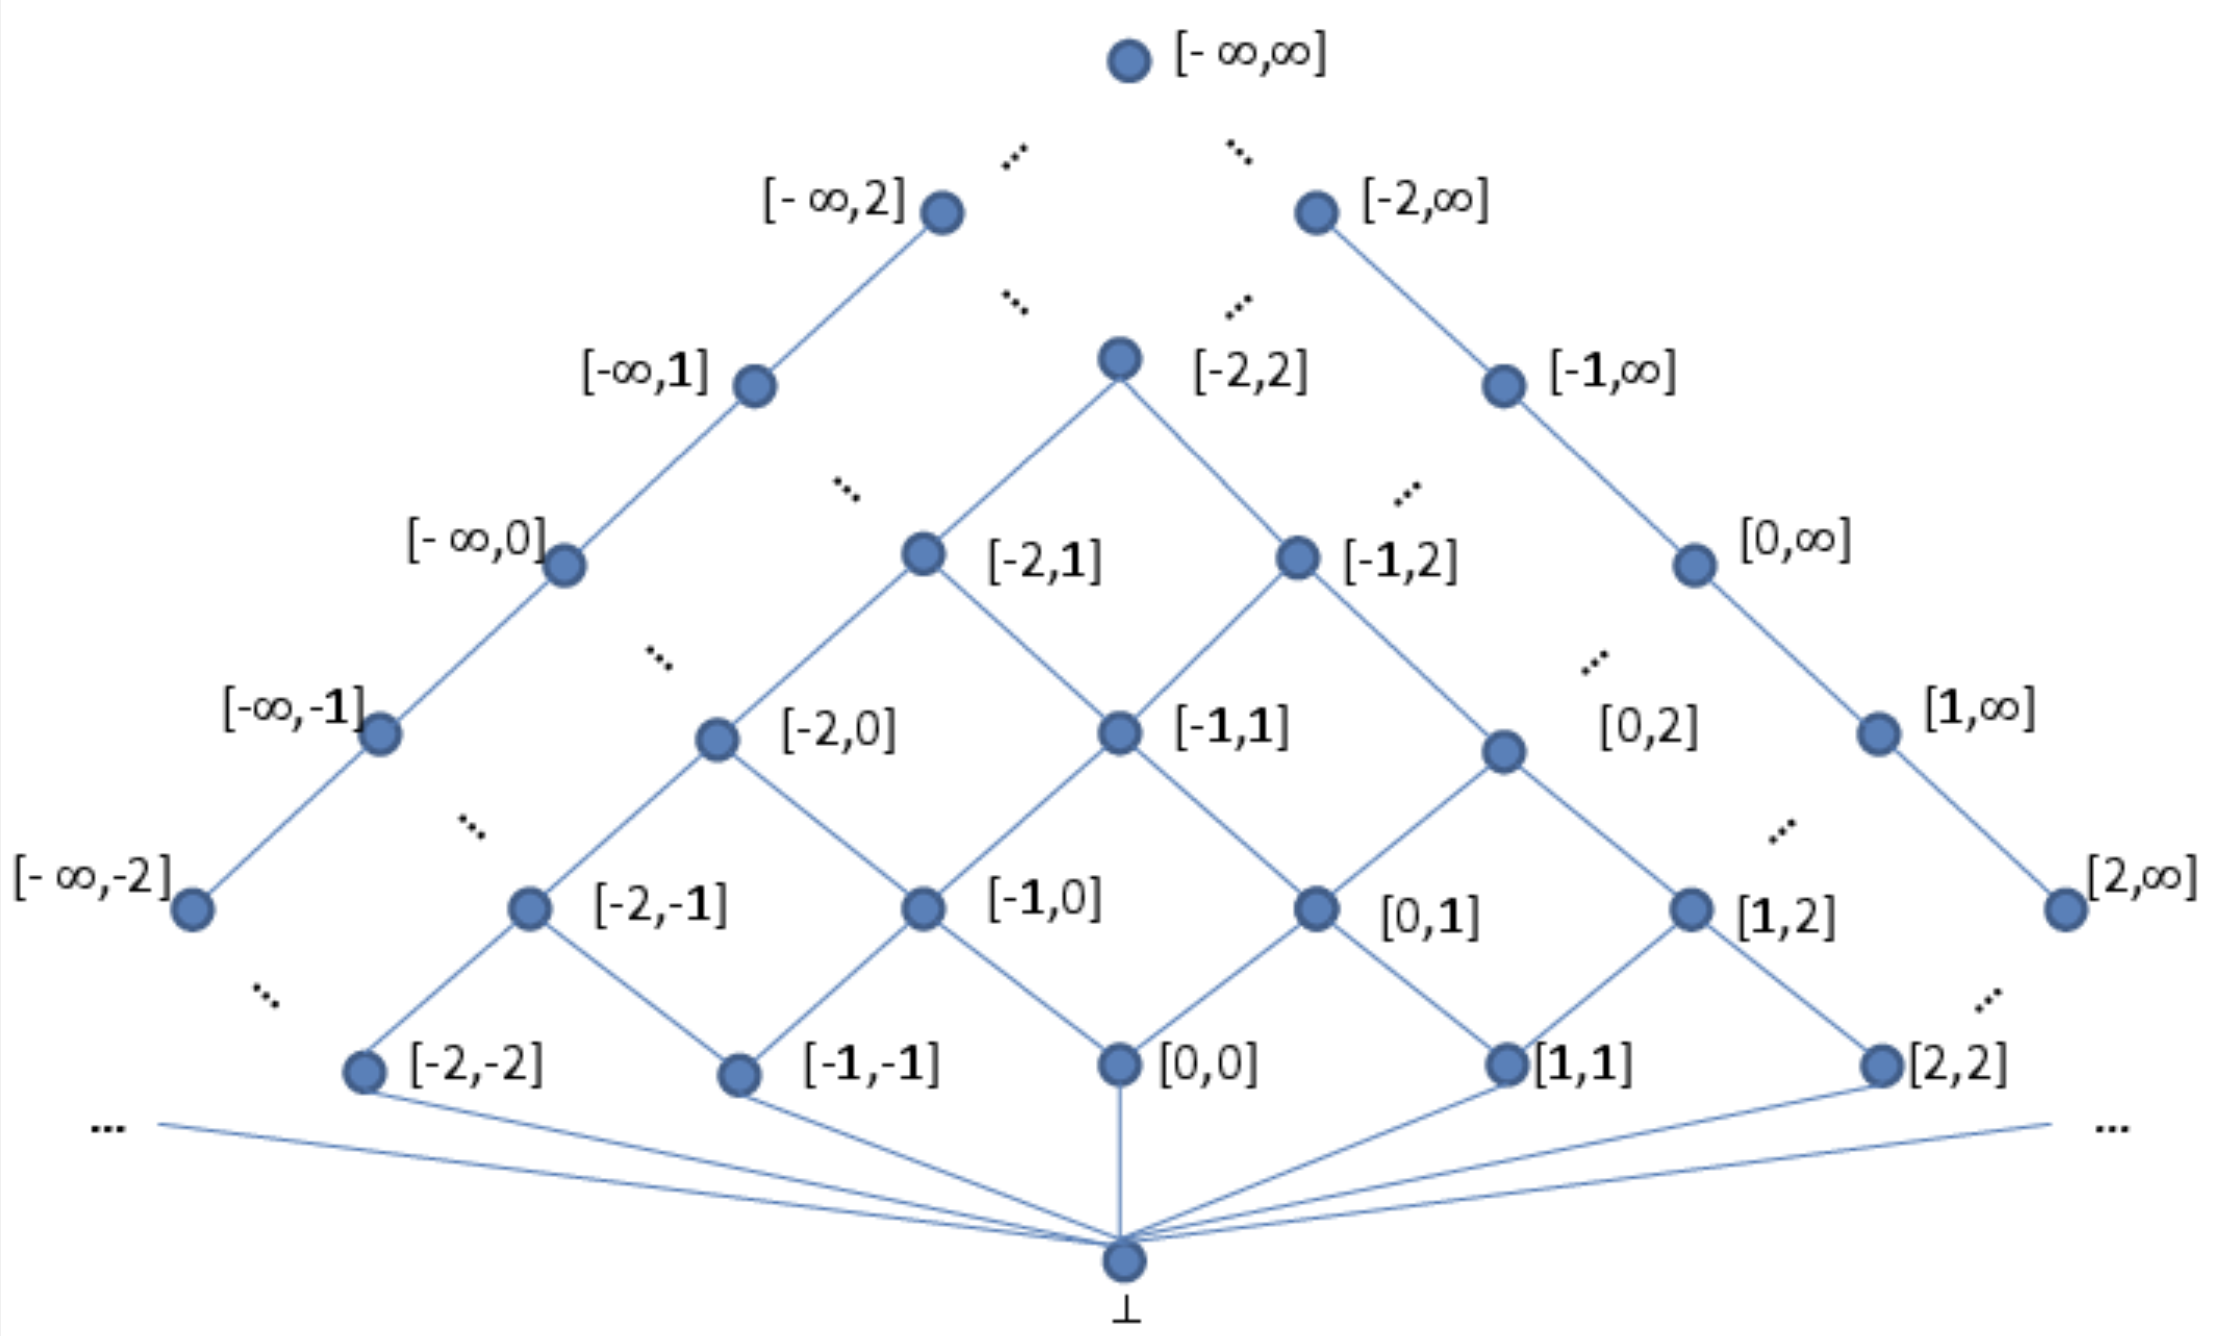
\includegraphics[width=0.8\columnwidth]{assets/interval_domain}
\end{center}

When we have two abstract elements $A$ and $B$, we can join them to produce their (least) upper bound, denoted by $A \sqcup B$. For this we have to define the join operation. \\

With the interval abstraction we can have cases where we cannot reach a fixed point, e.g. loop that always counts up. To fix this we introduce the widening operator, it ensures termination at the expense of precision. If the bound of an interval is increasing, we simply go to $\infty$ instead of widening the interval multiple times.


\subsection{Mathematical Concepts}

\subsubsection{Structures}

A partial order is a binary relation $\sqsubseteq \; \subseteq \; L \times L$ on a set $L$ with the properties of being reflexive, transitive and anti-symmetric. The intuition is that it captures implications between facts. Later, we will say that if $p \sqsubseteq q$, then $p$ is more precise than $q$. Given a poset, we can construct a Hasse diagram. \\

Given a poset $(L, \sqsubseteq)$, an element $\bot \in L$ is called the least element if it is smaller than all other elements of the poset. The greatest element $\top$ is defined analogous. The least and greatest elements may not exist, but if they do they are unique. \\

Given a poset $(L, \sqsubseteq)$ and $Y \subseteq L$, $u \in L$ is an upper bound of $Y$ if $\forall p \in Y: p \sqsubseteq u$. $\bigsqcup Y \in L$ is a least upper bound of $Y$ if it is an upper bound of $Y$ and $\bigsqcup Y \sqsubseteq u$ whenever $u$ is another upper bound of $Y$. We define the lower bound and greatest lower bound analogously. \\

A complete lattice $(L, \sqsubseteq, \bigsqcup)$ is a poset where $\bigsqcup Y$ and $\bigsqcap Y$ exist for any $Y \subseteq L$. The interval domain from above is a complete lattice.

\subsubsection{Functions}

A function $f: A \to B$ between two posets $(A, \sqsubseteq)$ and $(B, \leq)$ is increasing (monotone) if: 
$$\forall a, b \in A: a \sqsubseteq b \Rightarrow f(a) \leq f(b)$$

For a poset $(A, \sqsubseteq)$, a function $f: A \to A$, and element $a \in A$, $a$ is a fixed point iff $f(a) = a$. Further $a$ is a post-fixedpoint iff $f(a) \sqsubseteq a$. The set of all fixed points is denoted by Fix(f) and the set of all post-fixedpoints is denoted by Red(f). \\

For a poset $(A, \sqsubseteq)$ and a function $f: A \to A$, we say that $\text{lfp} \sqsubseteq f \in A$ is a least fixed point of $f$ if $\text{lfp} \sqsubseteq f$ is a fixed point and $\forall a \in A: a = f(a) \Rightarrow \text{lfp} \sqsubseteq f \sqsubseteq a$.

\begin{center}
	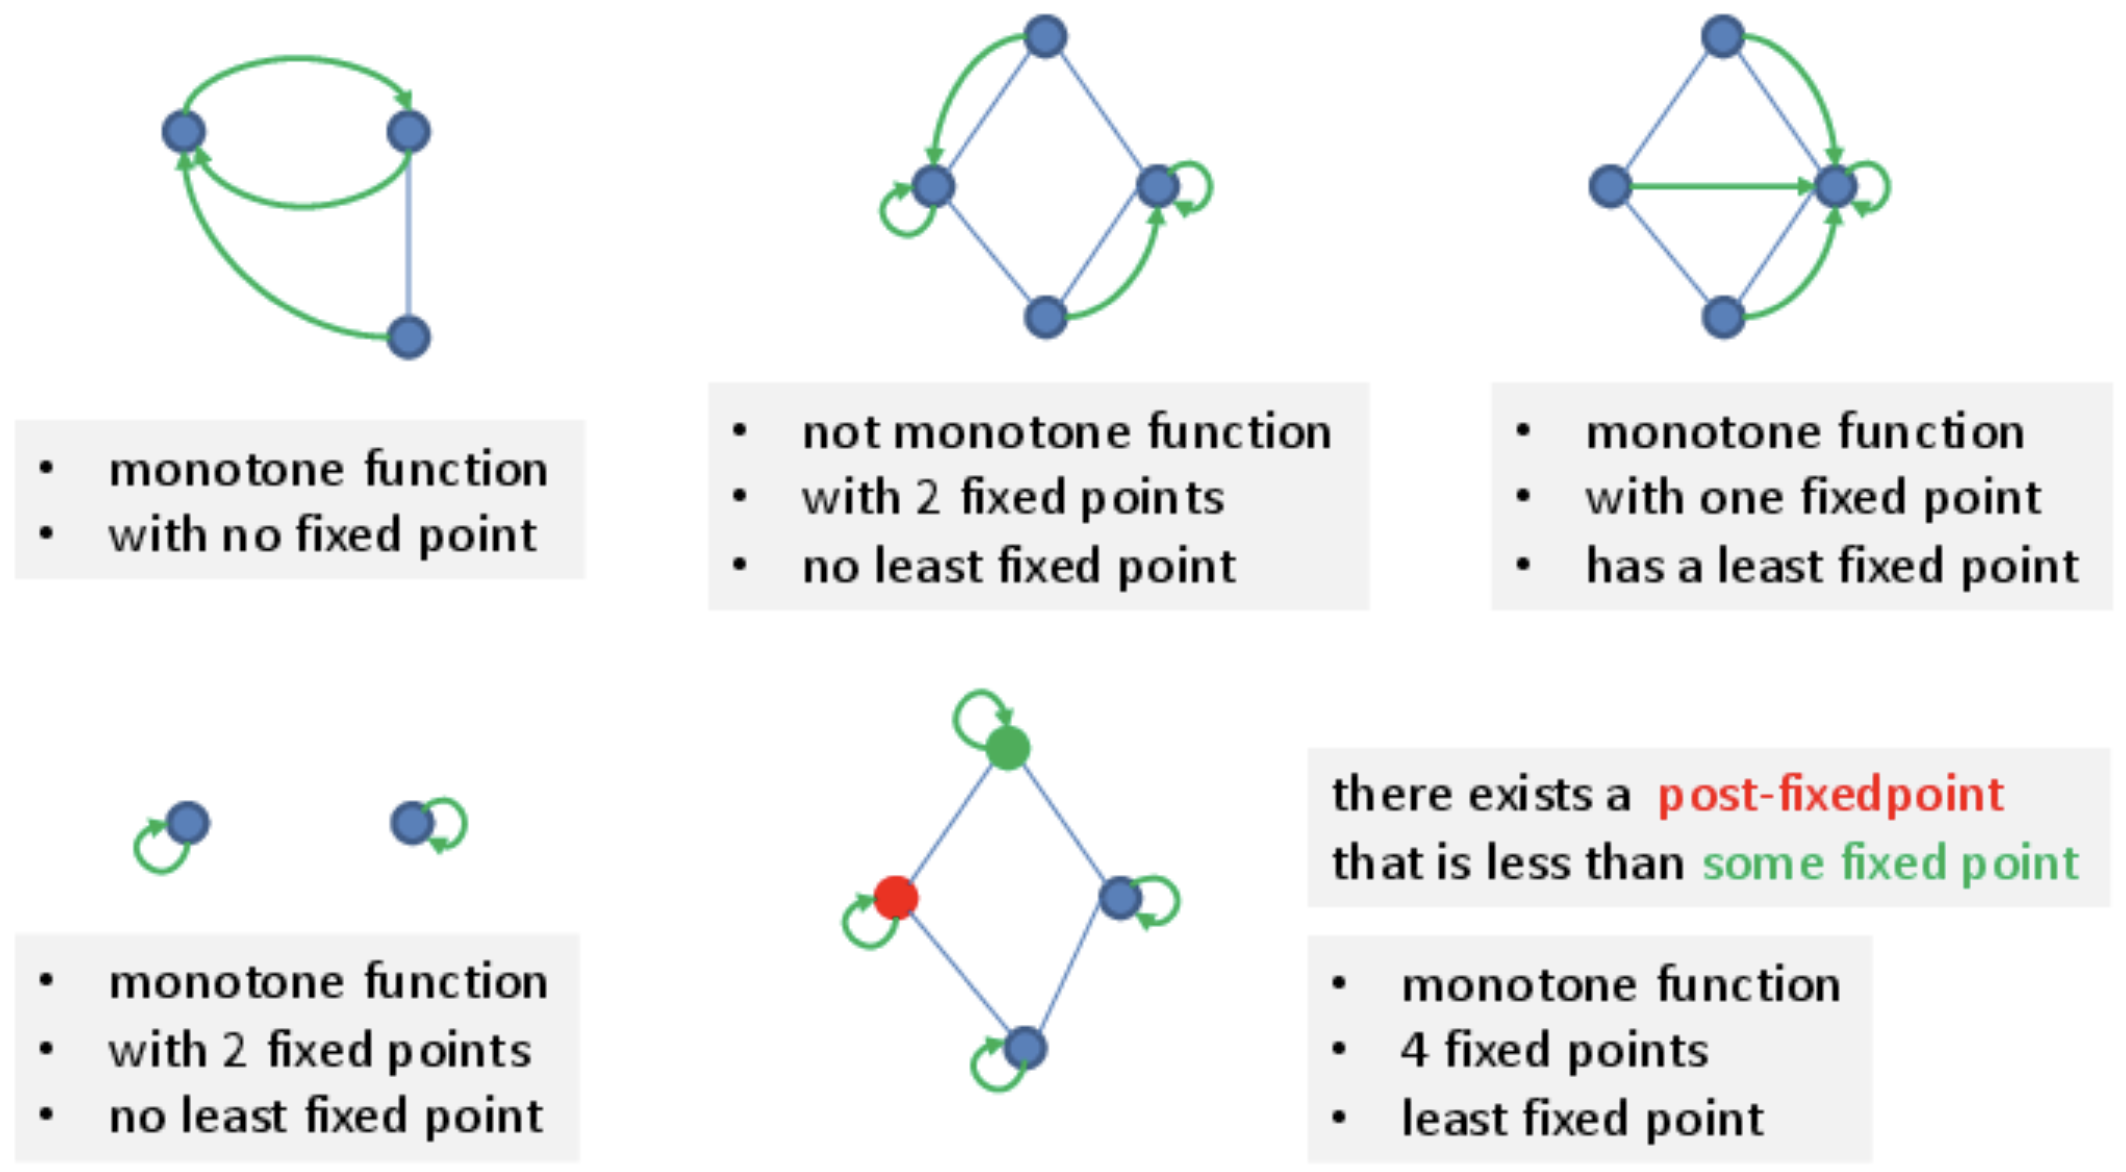
\includegraphics[width=\columnwidth]{assets/fixed_points}
\end{center}

If $(A, \sqsubseteq), \bigsqcup, \bigsqcap, \bot, \top)$ is a complete lattice and $f: A \to A$ is a monotone function, then $\text{lfp} \sqsubseteq f$ exists and $\text{lfp} \sqsubseteq f = \bigsqcap \text{Red}(f) \in \text{Fix}(f)$. \\

Given a poset of finite height, a least element $\bot$, a monotone $f$. Then the iterates $f^0(\bot), f^1(\bot), f^2(\bot), ...$ form an increasing squenece which eventually stabilizes.
$$\text{lfp} \sqsubseteq f = f^n(\bot)$$

\subsubsection{Approximating Functions}

Let $[[P]]$ be the set of reachable states of a program $P$. Let function $F$ be ($I$ is the initial state and $\to$ is the transition relation) :
$$F(S) = I \cup \{c' \, | \,�c \in S \land c \to c' \}$$

Then, $[[P]]$ is a fixed point of $F$, in fact it is the least fixed point of $F$. In static program analysis we want to approximate a programming language. For this, we define a function $F^\#$ that approximates $F$. Then, using existing theorems, approximate the least fixed point of $F$ by computing the least fixed point of $F^\#$. \\

A function $F^\#: C \to C$ approximates $F: C \to C$ if: 
$$\forall x \in C: F(x) \sqsubseteq_c F^\#$$

If $F: C \to C$ and $F^\#: A \to A$, we need to connect the concrete $C$ and abstract $A$. We do this via two function $\alpha: C \to A$ (abstraction function) and $\gamma: A \to C$ (concretization function). If we know that $\alpha$ and $\gamma$ form a Galois Connections, then we can use the following definition of approximation:
$$\forall z \in A : \alpha (F(\gamma(z))) \sqsubseteq F^\#(z)$$

\begin{center}
	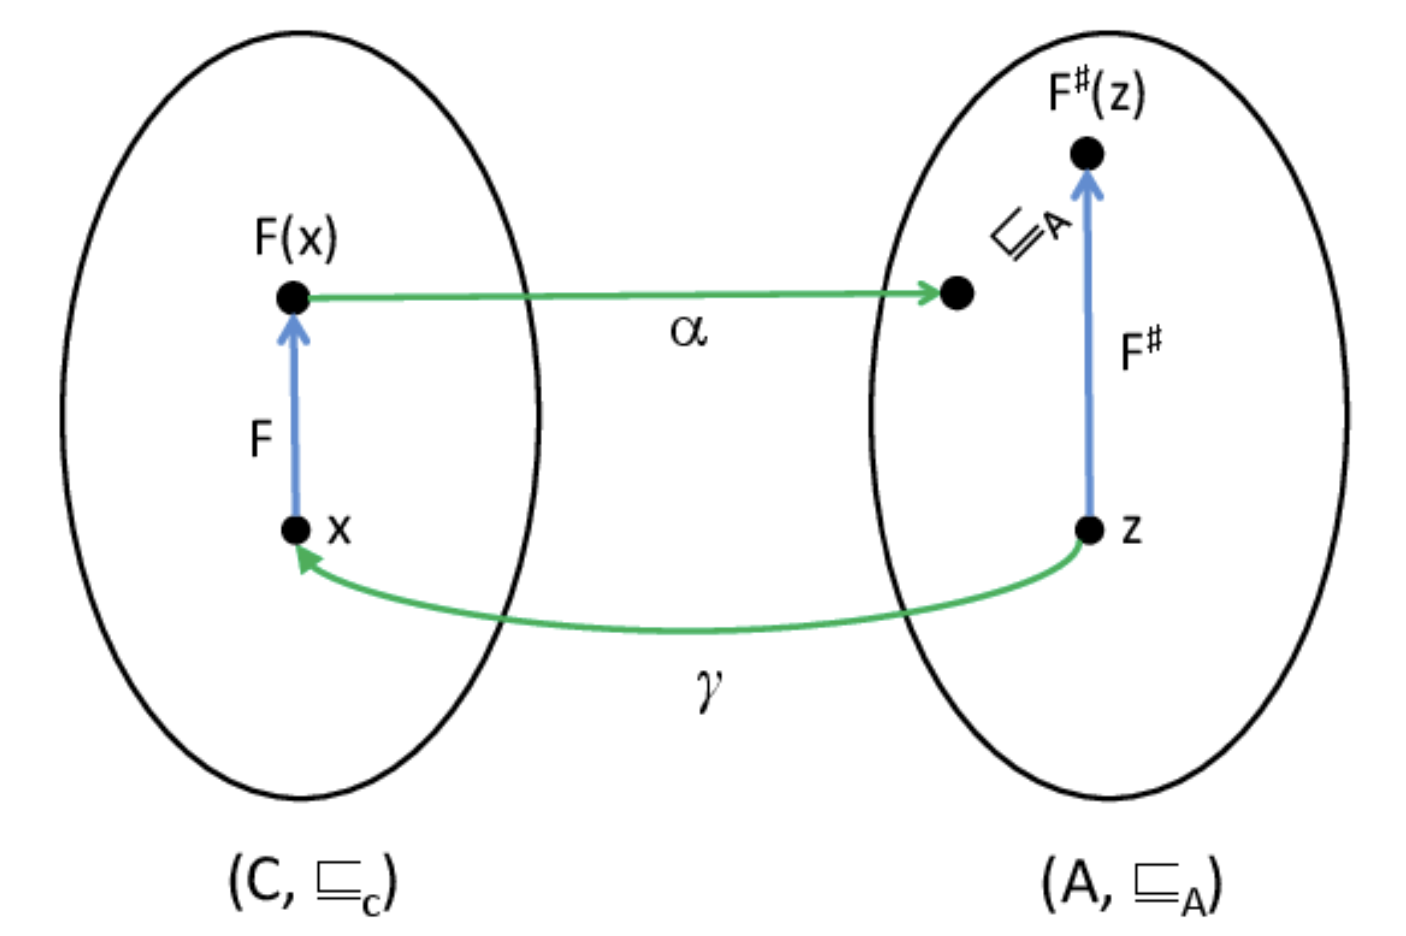
\includegraphics[width=0.7\columnwidth]{assets/approximation}
\end{center}

To approximate $F$, we can always define $F^\#(z) = \top$. This solution is always sound, however it is too imprecise. \\

The most precise approximation is given by $F^\#(z) = \alpha(F(\gamma(z)))$. The problem is that we often cannot implement such a $F^\#(z)$. However, we can come up with a $F^\#(z)$ that has the same behavior but a different implementation. Any such $F^\#(z)$ is referred to as the best transformer. \\

\textbf{Least Fixed Point Approximation} - If we have the following properties:
\begin{enumerate}
	\item monotone functions $F: C \to C$ and $F^\#: A \to A$
	\item $\alpha: C \to A$ and $\gamma: A \to A$ form a Galois Connection
	\item $\forall z \in A: \alpha(F(\gamma(z))) \sqsubseteq_A F^\#(z)$ (that is, $F^\#$ approximates $F$)
\end{enumerate}

Then $\alpha(\text{lfp}(F)) \sqsubseteq_A \text{lfp} (F^\#)$. This is important as it goes from local function approximation to global approximation. \\

If $\alpha$ and $\gamma$ do not form a Galois connection, then we can use the following definition of approximation: 
$$\forall z \in A : F(\gamma(z)) \sqsubseteq_C \gamma(F^\#(z))$$
\begin{center}
	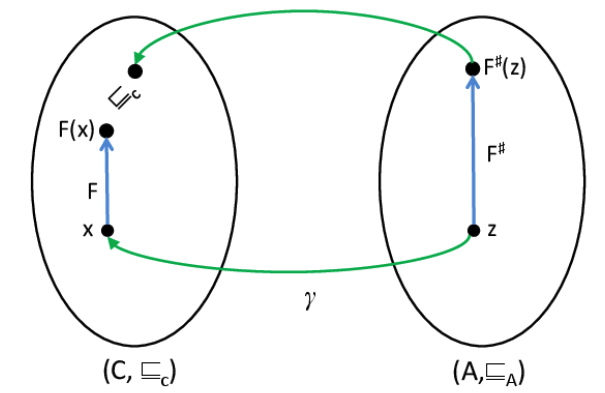
\includegraphics[width=0.7\columnwidth]{assets/approximation2}
\end{center}

If we have the following properties:
\begin{enumerate}
	\item monotone functions $F: C \to C$ and $F^\#: A \to A$
	\item $\gamma: A \to A$ is monotone
	\item $\forall z \in A : F(\gamma(z)) \sqsubseteq_C \gamma(F^\#(z))$ (that is, $F^\#$ approximates $F$)
\end{enumerate}

Then $\text{lfp}(F) \sqsubseteq_C \gamma(\text{lfp}(F^\#))$ \\

So what is $F^\#$ then? $F^\#$ is to be defined for the particular abstract domain $A$. The domain $A$ can be Sign, Parity, Interval, Polyhedra, and so on. In our setting, we simply keep a map from every label in the program to an abstract element in $A$. Then $F^\#$ simply updates the mapping from labels to abstract elements.
$$F^\#: (\text{Lab} \to A) \to (\text{Lab} \to A)$$


\subsection{Applications of Analysis: Intervals}

In this part, we will put these things together to build static analyzers. For this we first select a abstract domain, define the abstract semantics and then iterate the abstract transformer over a program until a fixed point is reached. \\

Our starting point is a domain where each element of the domain is a set of states. The domain of states is a complete lattice:
$$(\mathcal{P}(\Sigma), \subseteq, \cup, \cap, \emptyset, \Sigma) \qquad \Sigma = \text{Lab} \times \text{Store}$$

\subsubsection{Select Abstract Domain}

If we are interested in properties that involve the range of values that a variable can take, we can abstract the set of states into a map that captures the range of values each variable can take. \\

Let the interval domain be:
$$(L^i, \sqsubseteq_i, \sqcup_i, \sqcap_i, \bot_i, [-\infty, \infty])$$

We denote $\mathbb Z^\infty = \mathbb Z \cup \{-\infty, \infty\}$ and $L^i = \{ [x, y] \, | \, x, y \in \mathbb Z^\infty, x \leq y \} \cup \{ \bot_i \}$. Further we define a max and min function. Lastly, we can define the operations:
\begin{itemize}
	\item $[a, b] \sqsubseteq_i [c, d]$ if $c \leq a$ and $b \leq d$
	\item $[a, b] \sqcup_i [c, d] = [\text{min}(a, c), \text{max}(c, d)]$
	\item $[a, b] \sqcap_i [c, d] = \text{wdi}[\text{min}(a, c), \text{max}(c, d)]$ where wdi (well-defined interval) returns $[a, b]$ if $a \leq b$
\end{itemize}

The $L^i$ domain defines intervals, but to apply it we need to take program labels and program variables into account. Therefore, for programs, we use the domain: Lab $\to$ (Var $\to$ $L^i$). This domain is also a complete lattice. The operators are lifted directly to both domains.
$$\alpha_i: \mathcal P (\Sigma) \to (\text{Lab} \to (\text{Var} \to L^i))$$
$$\gamma_i: (\text{Lab} \to (\text{Var} \to L^i)) \to \mathcal P (\Sigma)$$

Using $\alpha_i$, we abstract a set of states into a map from program labels to interval ranges for each variable. Using $\gamma_i$, we concretize the intervals maps to a set of states.

\subsubsection{Define Abstract Semantics}

We still need to compute $\alpha_i [[P]]$ or an over approximation of it. We want a function: 
$$F^i: (\text{Lab} \to (\text{Var} \to L^i)) \to (\text{Lab} \to (\text{Var} \to L^i))$$

With the property $\alpha_i (\text{lfp F}) \sqsubseteq \text{lfp} F^i$. \\

\textbf{Generic Template for $F^\#$}:
$$F^\# (m) l = \begin{cases}
	\top & \text{if } l \text{ is initial label} \\
	\bigsqcup_{(l', \text{action}, l)} [[\text{action}]](m(l')) & \text{otherwise}
\end{cases}$$

This results in the following $F^i$ which approximates the best transformer but only works on the abstract domain.
$$F^i (m) l = \begin{cases}
	\lambda v. [-\infty, \infty] & \text{if } l \text{ is initial label} \\
	\bigsqcup_{(l', \text{action}, l)} [[\text{action}]]_i (m(l')) & \text{otherwise}
\end{cases}$$

$(l', \text{action}, l)$ are the edges in the CFG, an example could be $(1, \text{ x := 5}, \, 2)$. Next we would need to define all the effects for these. 
\begin{center}
	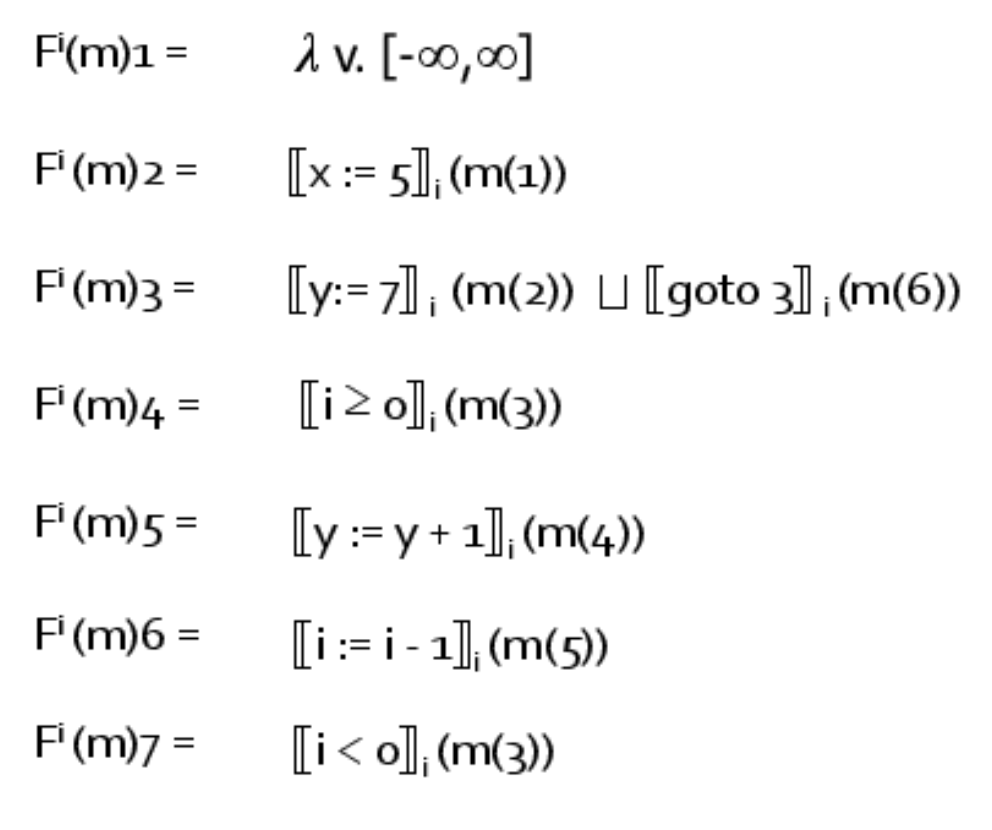
\includegraphics[width=0.6\columnwidth]{assets/effects}
\end{center}

\subsubsection{Iterate the Transformer}

In the final step, we know compute the least fixed point for a given program. However, especially with loops we can encounter the problem where a variable indefinitely changes (counts up or down). To avoid this we have to use widening. The widening operator $\nabla: L \times L \to L$ is defined as:
\begin{itemize}
	\item $\forall a,b \in L: a \sqcup b \sqsubseteq a \nabla b$
	\item if $x^0 \sqsubseteq x^1 \sqsubseteq ... \sqsubseteq x^n \sqsubseteq ...$ is an increasing sequence then $y^0 \sqsubseteq y^1 \sqsubseteq ... \sqsubseteq y^n$ stabilizes after a finite number of steps
\end{itemize}

Note that widening is completely independent of $F^i$, similar to join it is defined for a specific domain. If $\nabla, F$ are monotone then the sequence $y^0 = \bot, y^1 = y^0 \nabla F(y^0), ...$ will stabilize after a finite number of steps $n$ with $y^n$ being a post-fixed point of $F$. \\

For the interval domain, we define the widening operator $\nabla_i$ as $[a, b] \nabla_i [c, d] = [e, f]$ where $e = -\infty$ if $c < a$ and $f = \infty$ if $b < d$. \\

Iteration does not have to be in-order, there is also chaotic (asynchronous) iteration.


\subsection{Applications of Analysis: Pointers}

Pointer and Alias Analysis is fundamental to reasoning about heap manipulation programs. First we define the concrete store:
\begin{itemize}
	\item Objs is the set of all possible objects
	\item PtrVal = Objs $\cup \, \{$null$\}$
	\item $p \in \text{PrimEnv} : \text{Var} \to Z$
	\item $r \in \text{PtrEnv} : \text{PtrVar} \to \text{PtrVal}$
	\item $h \in \text{Heap} : \text{Objs} \to (\text{Field} \to \{ \text{PtrVal} \cup Z \})$
\end{itemize}

A store is now: 
$$\sigma = <p, r, h> \in \text{Store} = \text{PrimEnv} \times \text{PtrEnv} \times \text{Heap}$$

Before the store was only $p$. As before we have: 
$$\Sigma = \text{Lab} \times \text{Store}$$

Aliases are two pointers p and q that point to the same object. A points-to pair (p, A) means that p holds the address of object A. If (p, A) and (r, A) are points-to pairs, then p and r are aliases.\\

A program can create an unbounded number of objects. Therefore we need to use some abstraction when allocating a new object. That is, we need some static naming scheme for dynamically allocated objects. \\

Allocation sites divide the heap into a fixed partition based on the statement label. All objects allocated at the same program point (label) get represented by a single abstract object.
\begin{center}
	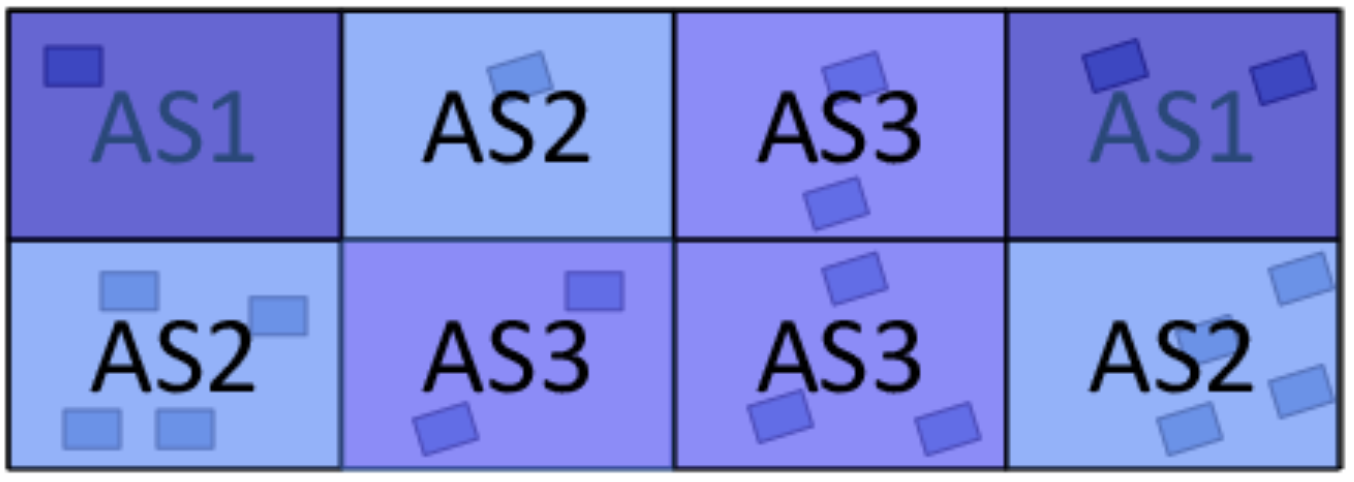
\includegraphics[width=0.8\columnwidth]{assets/allocation_sites}
\end{center}

If this is too imprecise, we can also use the calling context. If we use allocation sites (labels), we can now define the abstract objects as:
$$\text{AbsObj} = \{ l \,|\, \text{statement is p := alloc}^l \}$$

That is, this is just those labels in the program where allocation of an object occurs. Here alloc$^l$ is just the name of the allocation instruction.

\subsubsection{Flow Sensitive Pointer Analysis}

This type of analysis respects the program control flow. This leads to a separate set of points-to pairs for every program point. Further, the set at a program point represents possible maybe-aliases on some path from entry to the program point. \\

We use the same step-by-step approach as before. The abstract domain is a complete lattice:
\begin{align*}
	\text{Labs} \to ( \; &(\text{PtrVar} \to \mathcal P ( \text{AbsObj})) \; \times \\
	&( \text{AbsObj} \times \text{Field} \to \mathcal P (\text{AbsObj})) \; )
\end{align*}

The abstract domain keeps two maps at every program label. The first one contains a mapping from a pointer variable to a set of abstract objects. The second map contains a mapping from the fields of abstract objects to the set of abstract objects they point to. Since this lattice is of finite height, we will not need widening. $\sqsubseteq, \sqcup, \sqcap, \bot, \top$ are all lifted appropriately. \\

Using $\alpha$, we abstract a set of states into the two kinds of maps. Similarly, using $\gamma$, we concretize the pointer maps to a set of states. \\

We now need to define the effect of program statements manipulating pointers on the abstract domain. It can be summarized as:
\begin{center}
	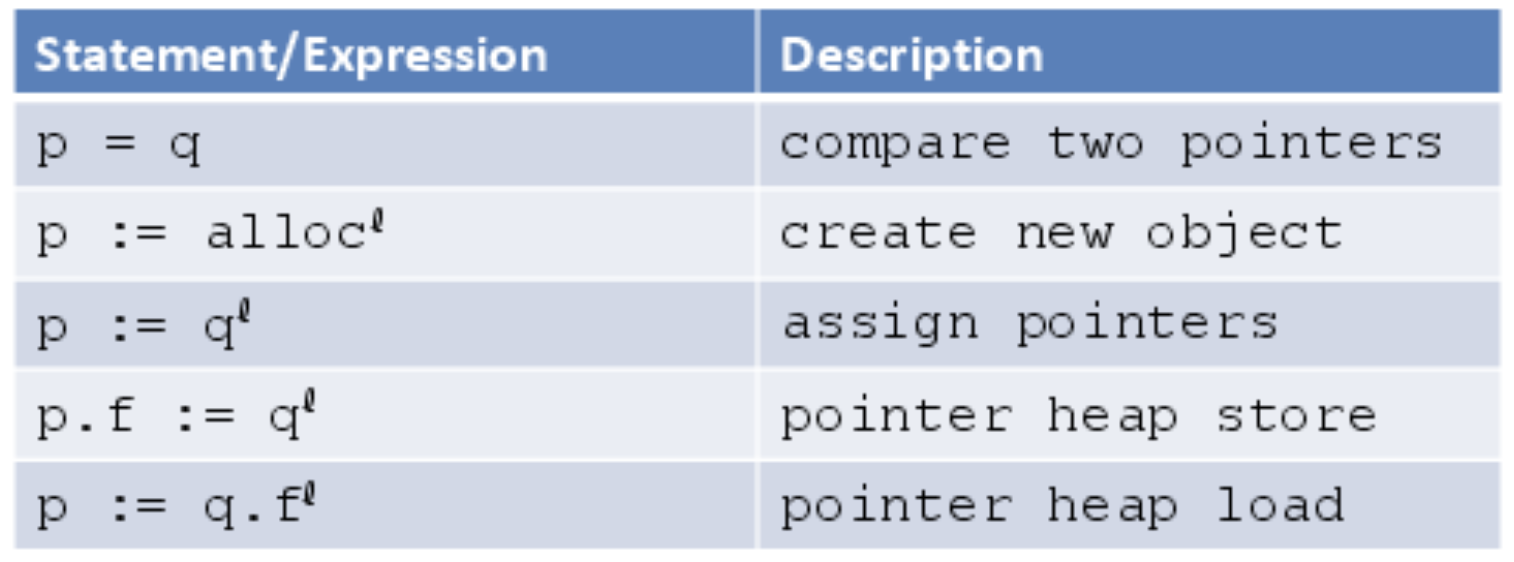
\includegraphics[width=\columnwidth]{assets/transformers}
\end{center}

Let ustake a look at the most tricky one, pointer heap store. Given \texttt{p.f := q} and \texttt{p $\to$ \{A\}}, \texttt{A.f $\to$ \{B\}}, and \texttt{q $\to$ \{C\}}. Is \texttt{A.f $\to$ \{C\}} the correct result? No, it is not. The correct solution would be \texttt{A.f $\to$ \{B, C\}}, this is called weak updates.


\subsubsection{Flow Insensitive Pointer Analysis}

This type of analysis assumes all execution orders are possible, it abstracts away order between statements. This is good for concurrency and is scalable, but it may be too imprecise. \\

The abstract domain does not keep information per label, essentially ignoring the control flow of the program.
\begin{align*}
	&(\text{PtrVar} \to \mathcal P ( \text{AbsObj})) \; \times \\
	&( \text{AbsObj} \times \text{Field} \to \mathcal P (\text{AbsObj}))
\end{align*}

To account for the loss of control-flow, all updates have to be weak. This can lead to very imprecise results. To avoid this, we can initialize local variables with \texttt{null} instead of $\top$.


\subsection{Application of Analysis: \\ Static Concurrency Checker}

Another use case is to check if parallel algorithms are deterministic. However, since proving determinism is hard, we prove a stronger property. We prove data-race freedom. \\

For static analysis there are three sources of unboundedness we have to deal with. These are the heap, the range of array indices, and the number of threads. For the heap we can use flow-insensitive points-to analysis and for the range of array indices we use numerical abstraction. \\

We first perform sequential analysis on a per thread basis. We then take the cartesian product of these states and filter out all the ones that are not possible. Leaving us with the concrete program states. \\

Now, we can check the property we are interested in proving.
\section{Symbolic \& Concolic Execution}


If we compute the symbolic constraints per path, and then solve these constraints we will have all concrete inputs that explore all paths. This is the core idea of symbolic execution.

\begin{center}
	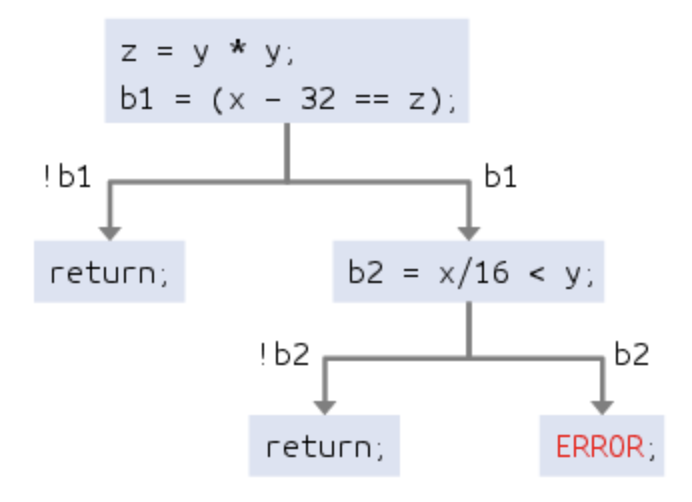
\includegraphics[width=0.5\columnwidth]{assets/path}
\end{center}

A symbolic store $\sigma$ maps variables to symbolic expressions, which are updated by assign statements. Path conditions $\pi$ are the conditions under which a path is taken. Combined we have a symbolic state per program point.
\begin{center}
	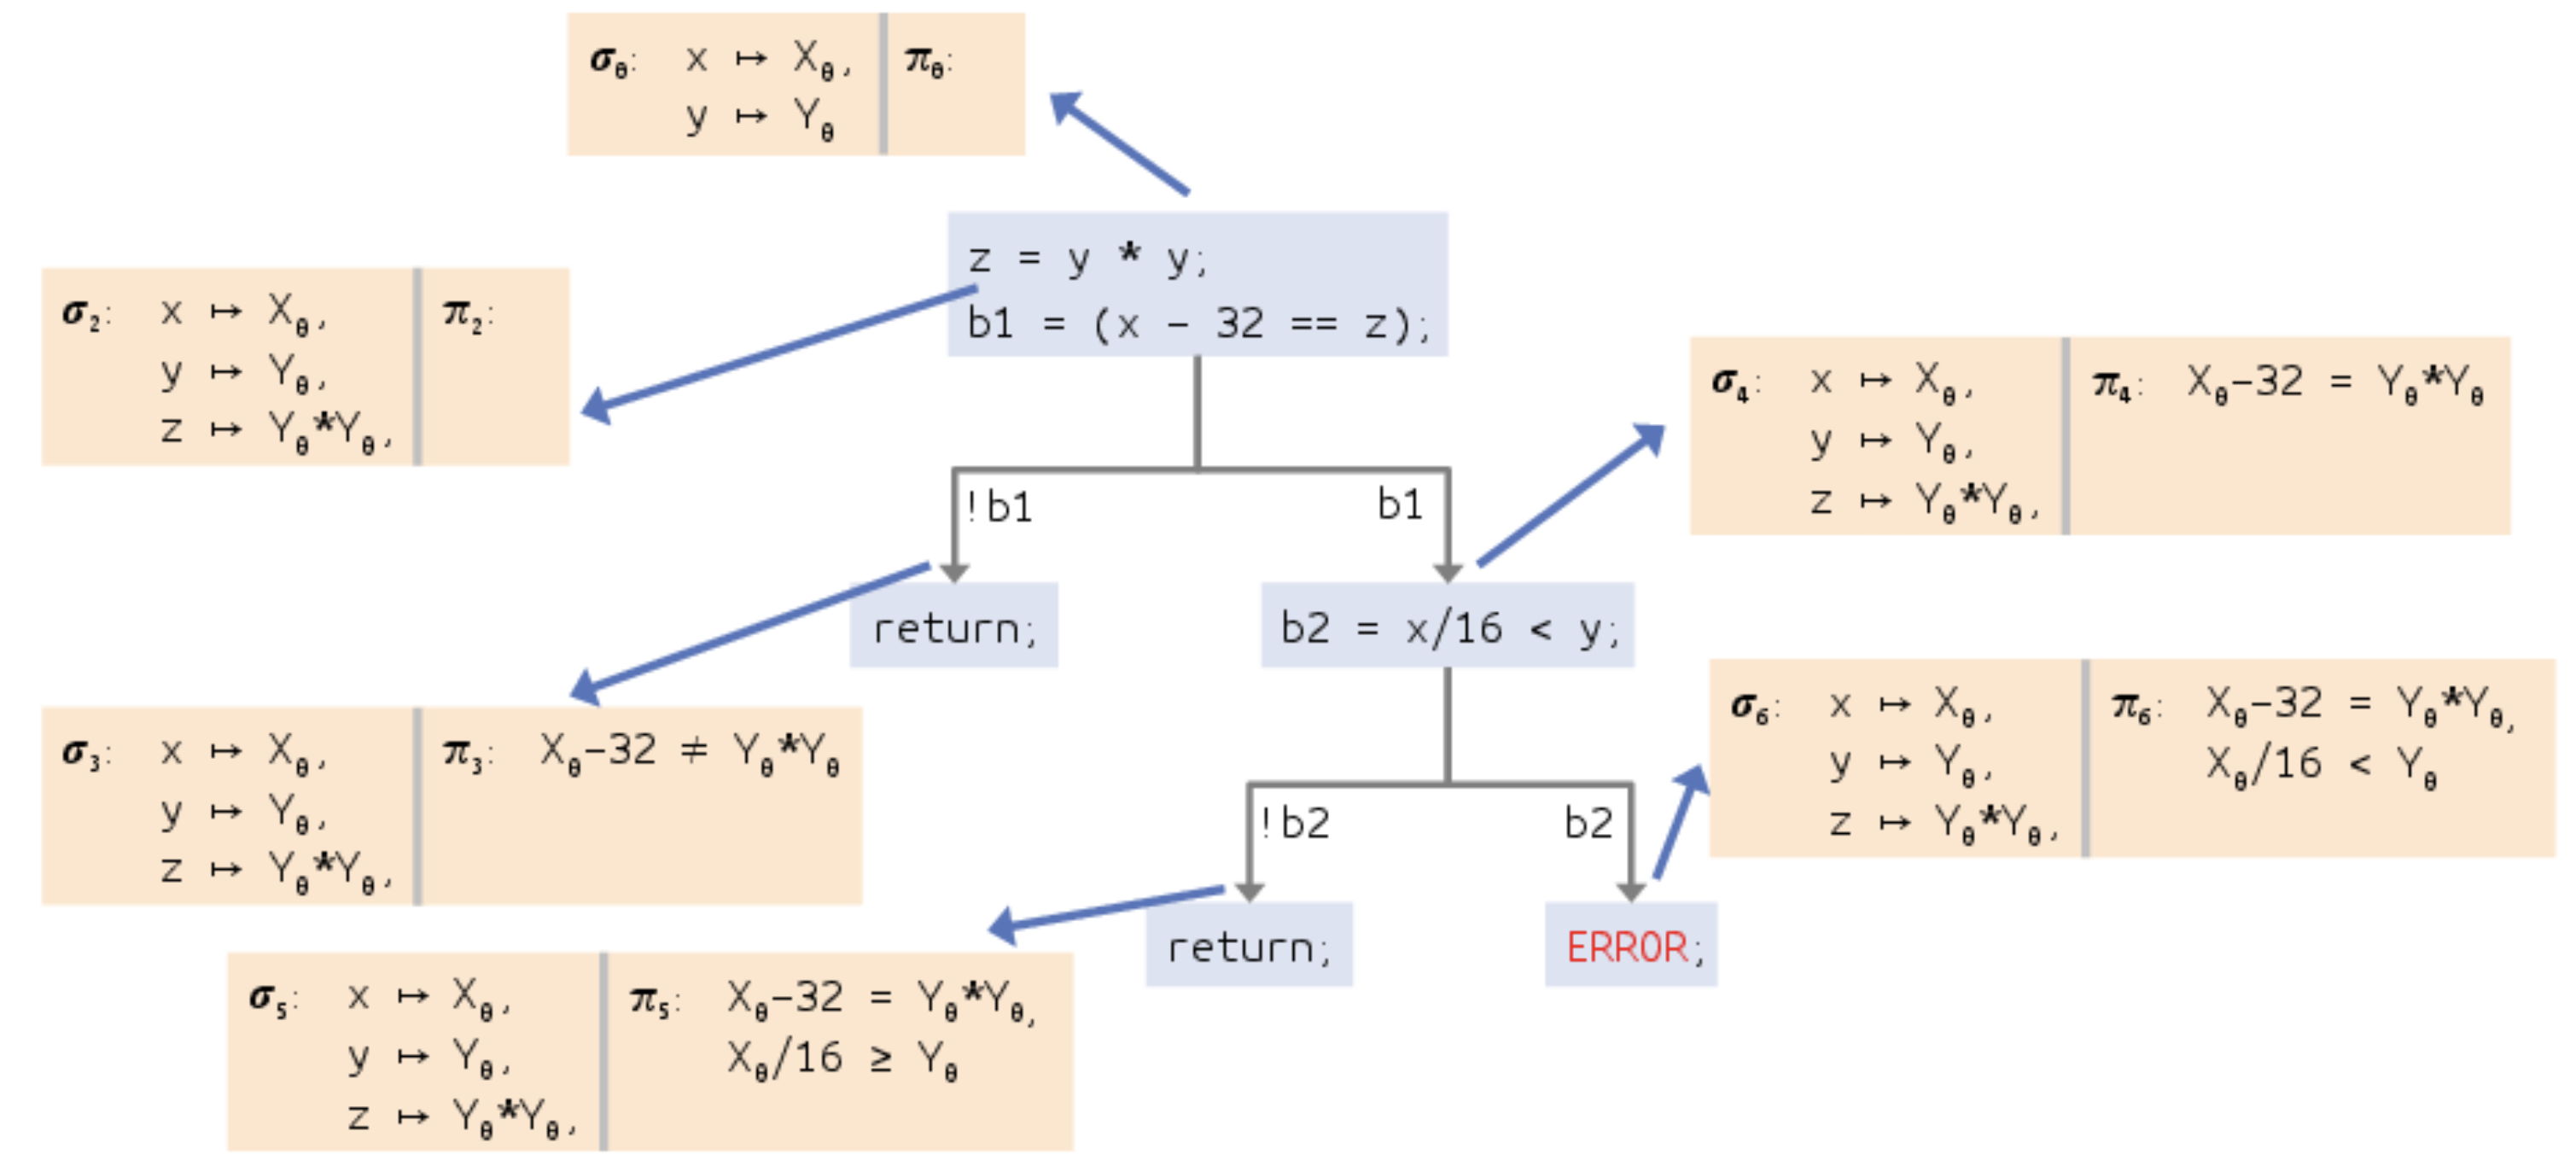
\includegraphics[width=\columnwidth]{assets/symbolic_execution}
\end{center}

Solving the final constraint sets, we can conclude which path will be taken for an input. \\

Eagerly exploring all paths up-front may include many infeasible paths and can be too time consuming. Symbolic execution engines therefore apply different exploration strategies. \\

SMT solvers combine SAT-solving with theory reasoning. They can produce models, satisfying assignments. However, there are limits. Many theories are not decidable, e.g. non-linear integers. Let us assume the solver fails to find a model for $b_1$ or $!b_1$, therefore we will not get concrete test inputs and cannot determine if the branch is infeasible. \\

Concolic execution combines concrete and symbolic execution. The high-level idea is that the concrete execution drives the symbolic one. Programs are executed with concrete inputs, but additionally maintain a symbolic state. Concrete values are used to simplify path conditions. \\

A concolic execution may not be able to explore all paths, but any additionally explored path increases the chances of uncovering bugs. We use concolic execution to expand sets of manually determined test inputs. \\

Symbolically executing native code is difficult if not impossible. Concolic execution can help by invoking the functions with concrete values. Still, it might not be able to explore all paths. \\

Further, one has to consider that symbolic expressions can become large, in particular along deep paths. Optimizations typically employed compilers are subexpression elimination and constant folding.


\subsection{Fuzzing and Symbolic Execution for Smart Contracts}

The idea behind fuzzing is to run programs on abnormal inputs (e.g. randomly generated). This should help finding potential exploits that attackers could use. \\

We want to find transactions that thoroughly explore the state space. The problem is the exponential number of block states. Both, symbolic execution and fuzzing, have their drawbacks. Imitation learning based fuzzers try to solve these problems.
\begin{center}
	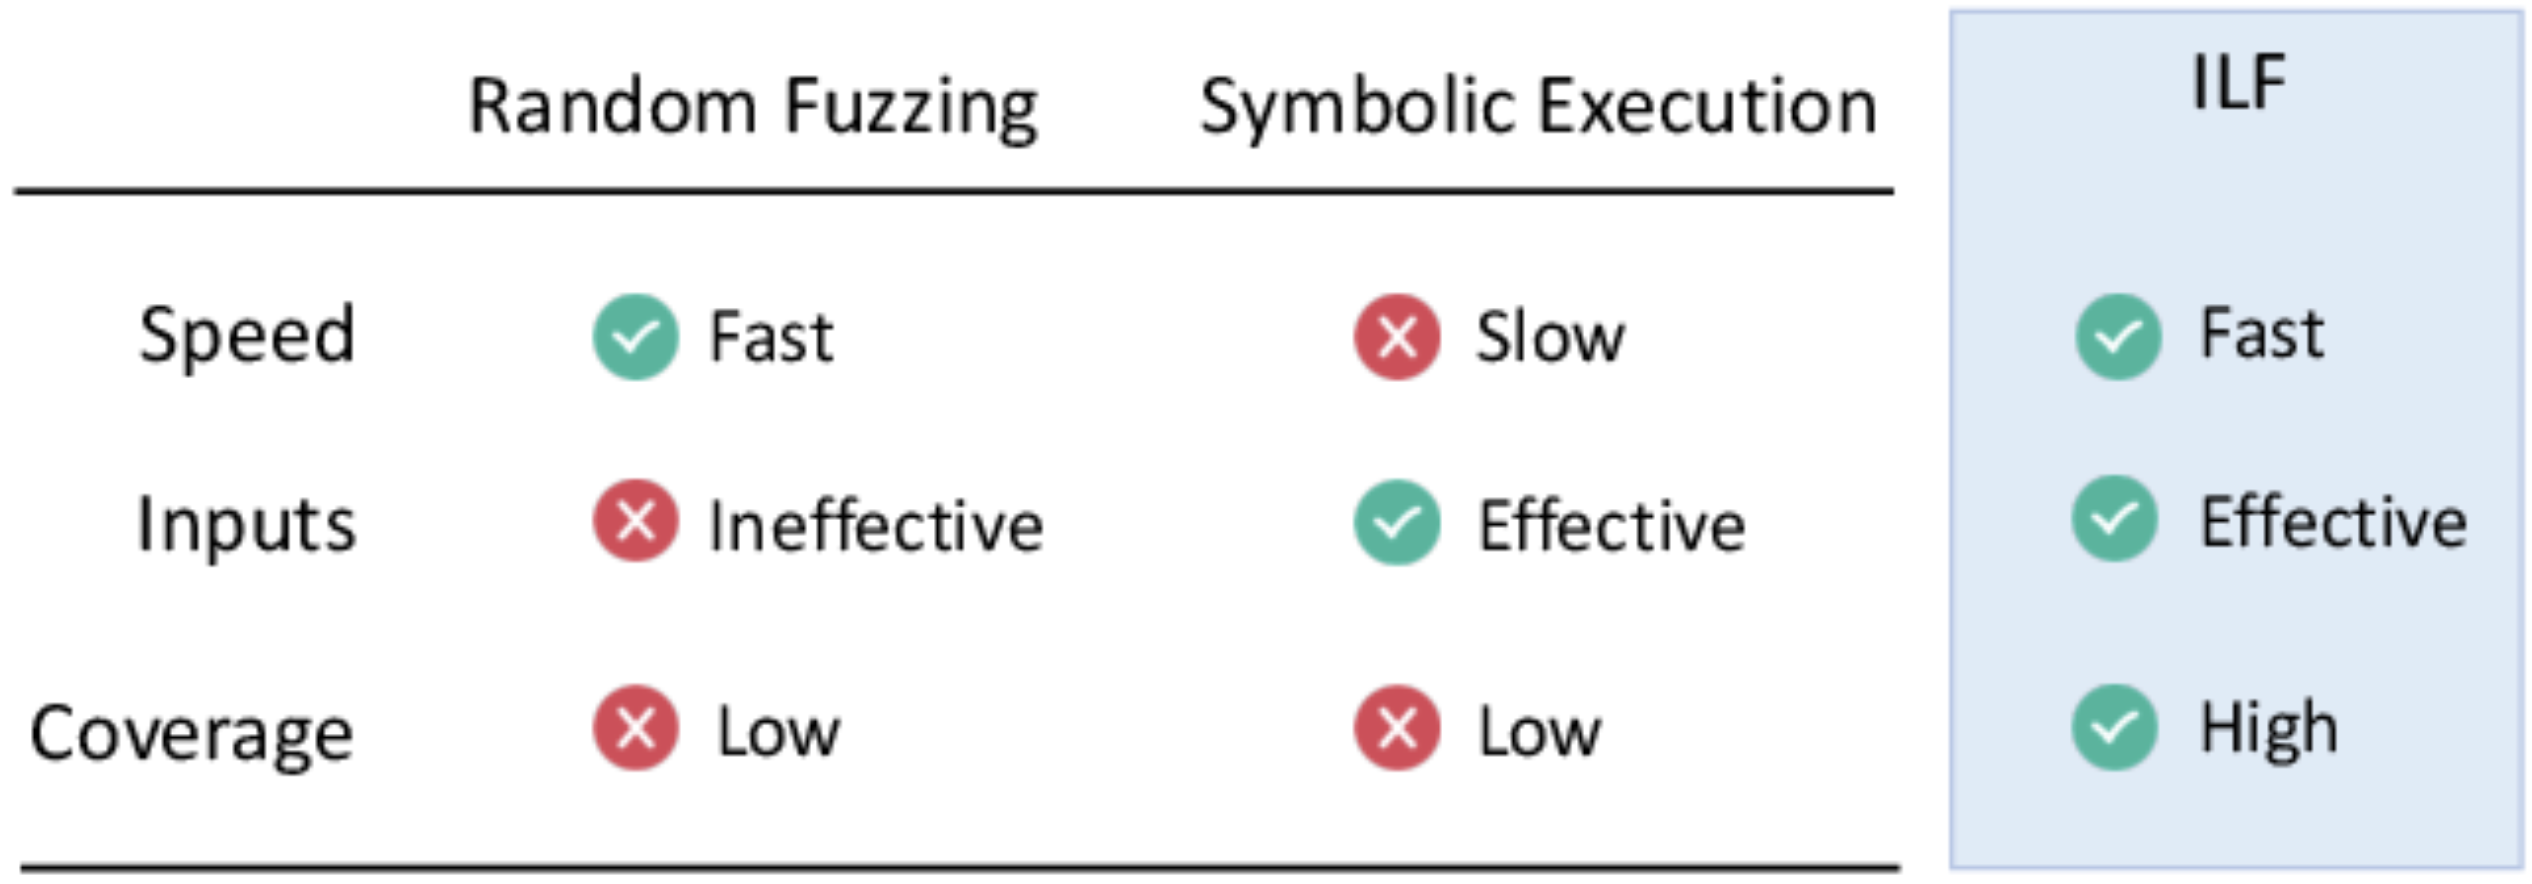
\includegraphics[width=0.9\columnwidth]{assets/fuzzing}
\end{center}

A neural network is used to learn to fuzz from symbolic execution.
\begin{center}
	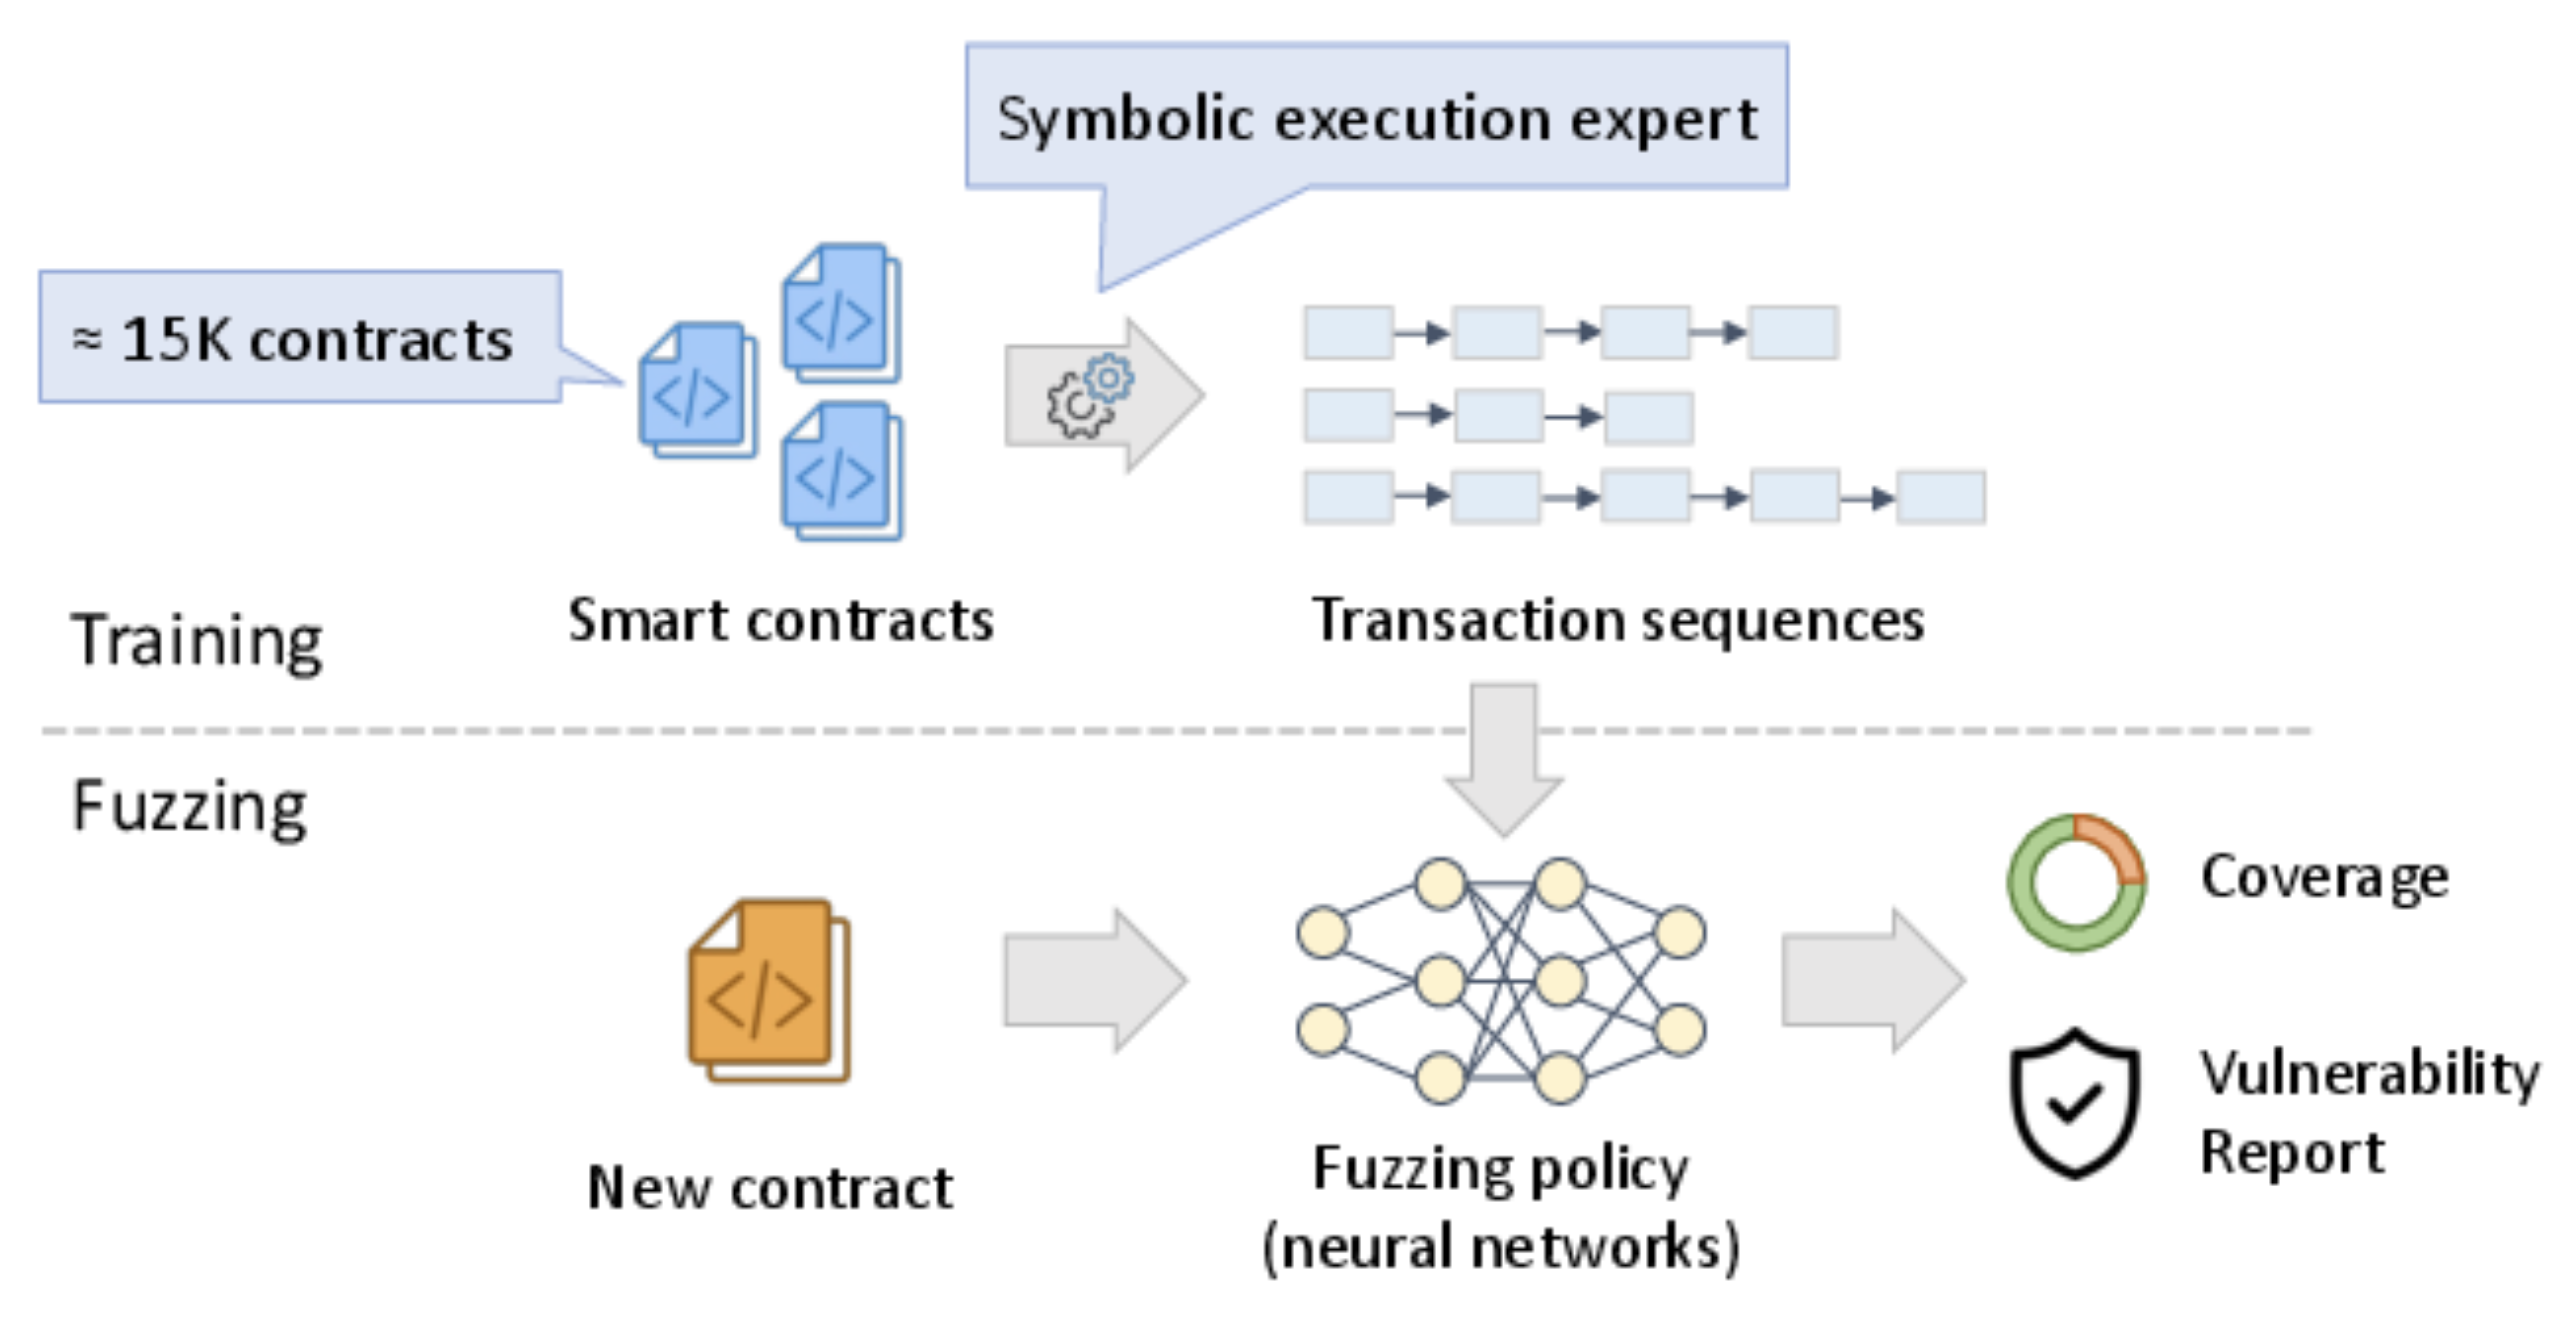
\includegraphics[width=0.9\columnwidth]{assets/ilf}
\end{center}

This approach performs better than anything comparable.
\section{Modeling and Specification}

Formal modeling use notations and tools from mathematics to be precise. Formal models enable the use of automatic analysis. They are good at finding ill-formed examples and checking properties. \\

Alloy is a formal modeling language based on set theory. An alloy model specifies a collection of constraints. The alloy analyzer takes the constraints of a model and tries to find a structure that satisfies them. There are three levels of abstraction in alloy: the object oriented paradigm, set theory, and atoms and relations.\\

There are four key ideas:
\begin{itemize}
	\item Everything is a relation. All data types and structures are relations. A key operator is dot join.
	\item Non-specialized logic. No special constructs for state machines, traces, synchronization, concurrency etc.
	\item Counterexamples \& Scope. Observations about design analysis: most assertions are wrong and most flaws have small counterexamples.
	\item Analysis by SAT. SAT is easy, so reduce the problem to SAT.
\end{itemize}


\subsection{Logic}

Atoms are alloy's primitive entities (indivisible, immutable and uninterpreted). Relations are use to associate atoms with one another. Every value in alloy logic is a relation.\\

Sets are unary relations, scalars are singleton sets and binary relations are sets of two columns. For these relations it holds that rows are unordered while columns are ordered but unnamed. Further, all relations are first order relations, meaning they cannot contains other relations (no set of sets).\\

We have the following constants: \texttt{none} is the empty set, \texttt{univ} is the universal set and \texttt{iden} is the identity relation.

\subsubsection{Operators}

\textbf{Set Operators}
\begin{center}
	\begin{tabular}{l l}
  		\texttt{+} & union \\
  		\texttt{\&} & intersection \\
  		\texttt{-} & difference \\
  		\texttt{in} & subset \\
  		\texttt{=} & equality \\
  		\texttt{->} & cross product
	\end{tabular}
\end{center}

\textbf{Join Operators}

\texttt{.}  dot join, column that is joind on is left out of the result\\
\texttt{[]} box join, \texttt{a.b.c[d] = d.(a.b.c)}\\

\textbf{Restriction and Override}
\begin{center}
	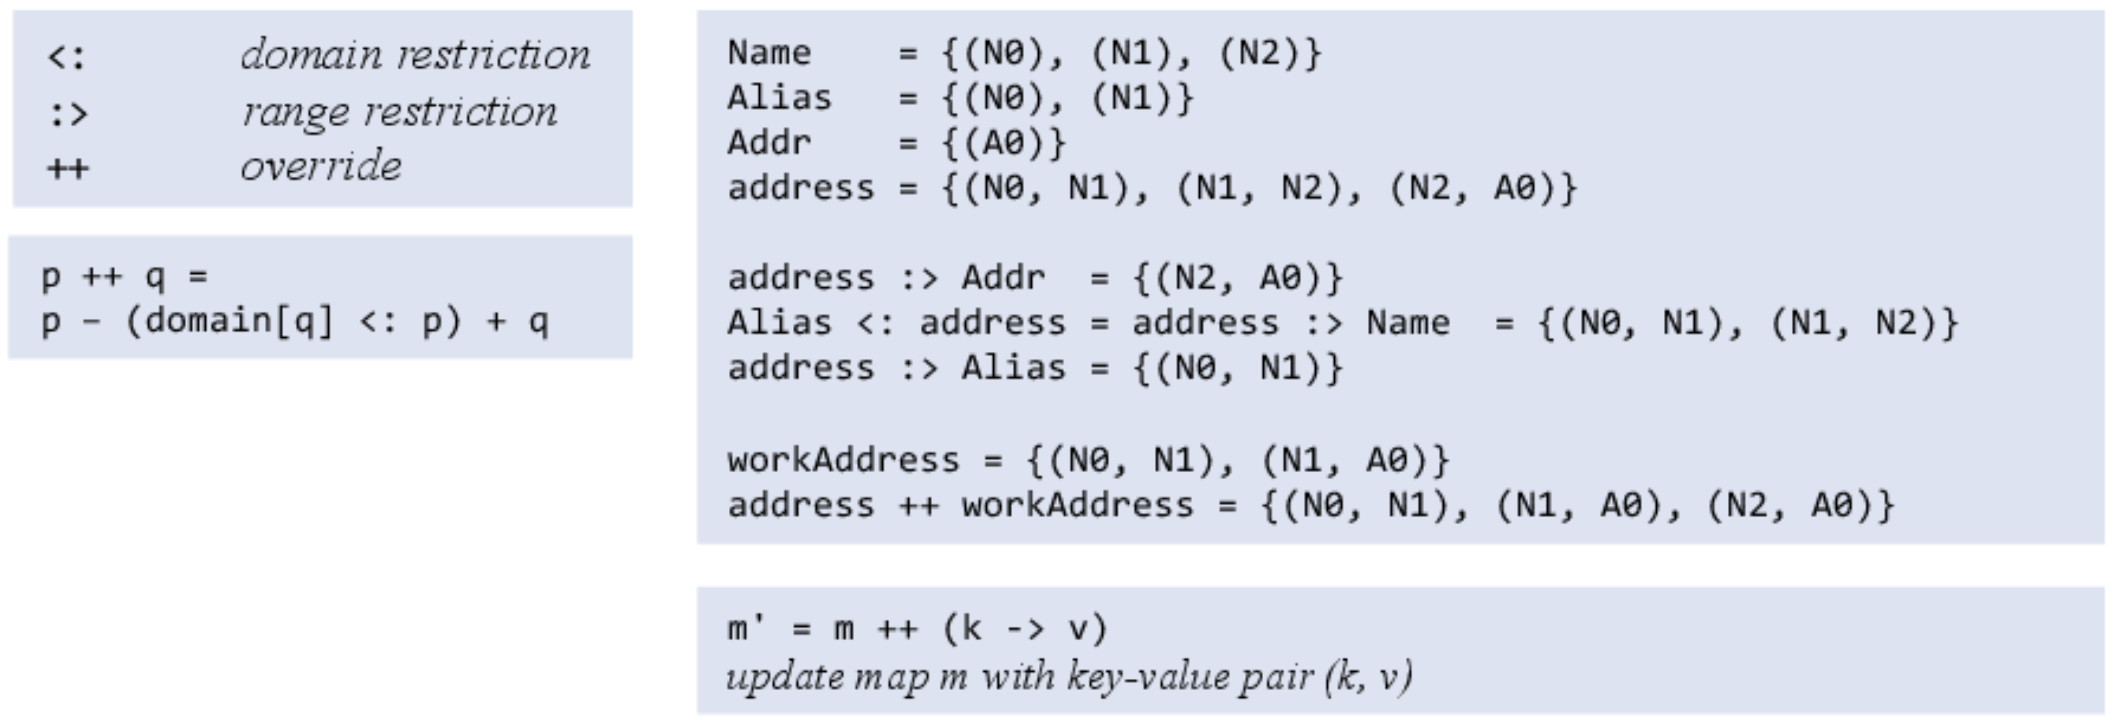
\includegraphics[width=\columnwidth]{assets/restriction}
\end{center}

\vspace{-8pt}
\textbf{Unary Operators}
\begin{center}
	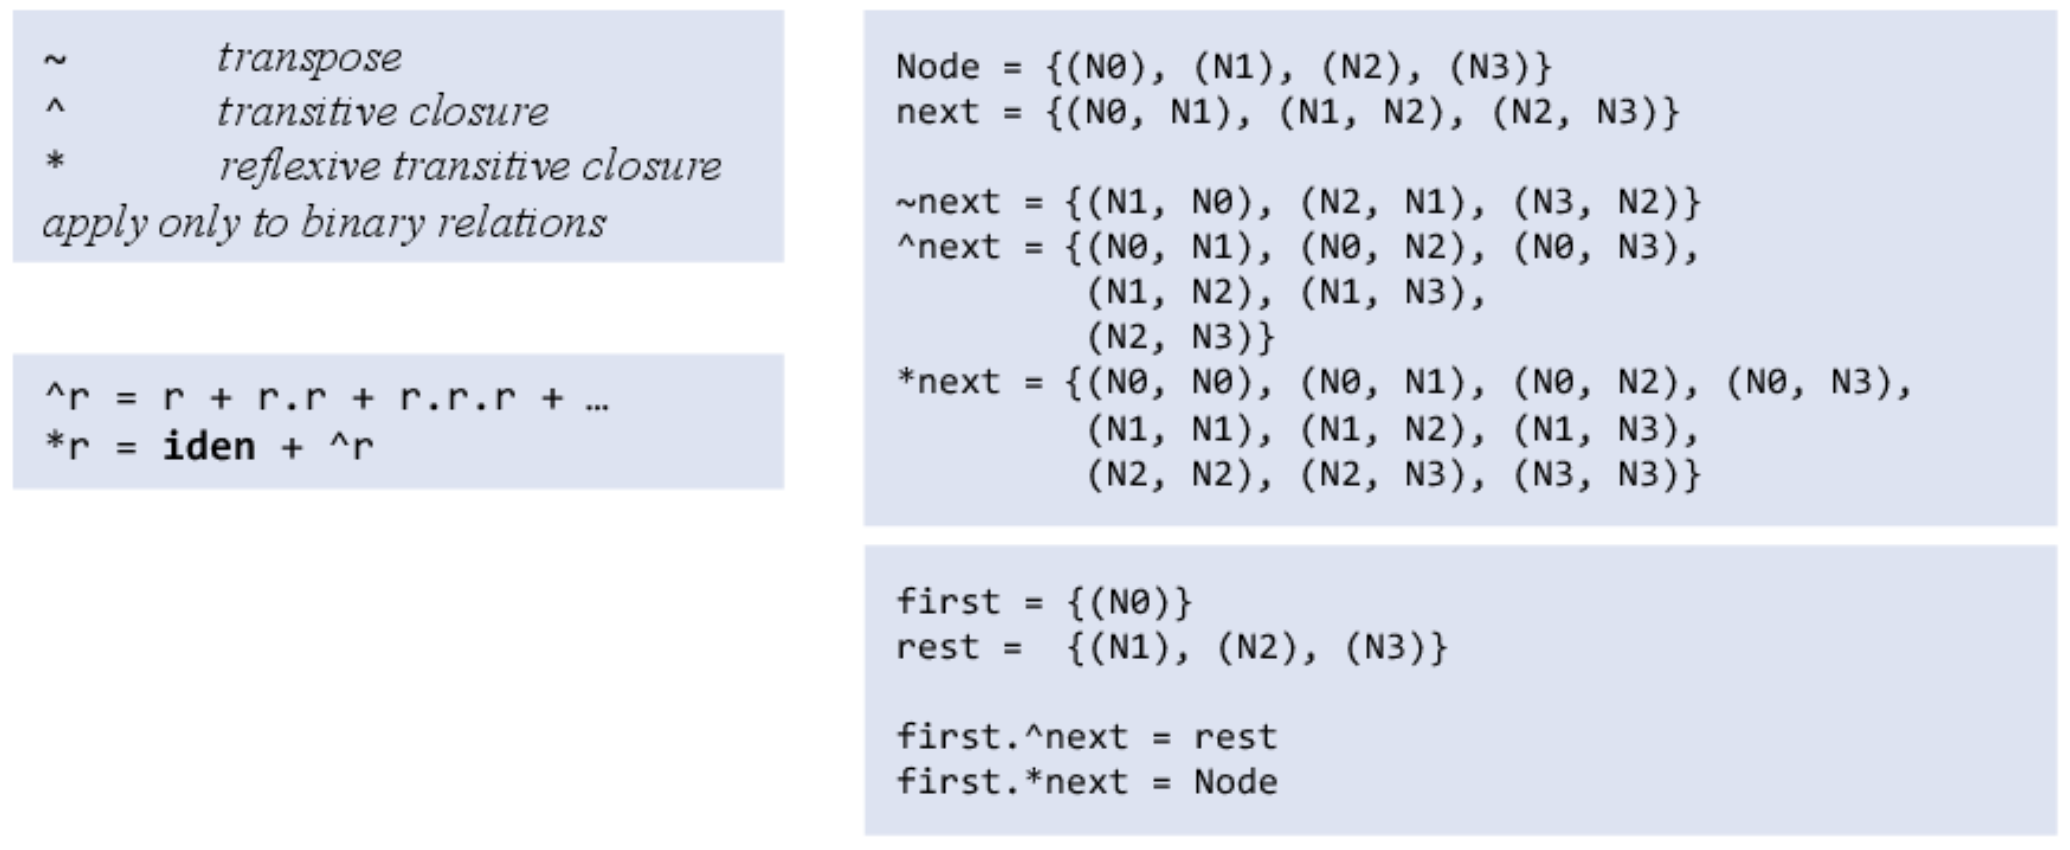
\includegraphics[width=\columnwidth]{assets/unary}
\end{center}

\vspace{-8pt}
\textbf{Boolean Operators}
\begin{center}
	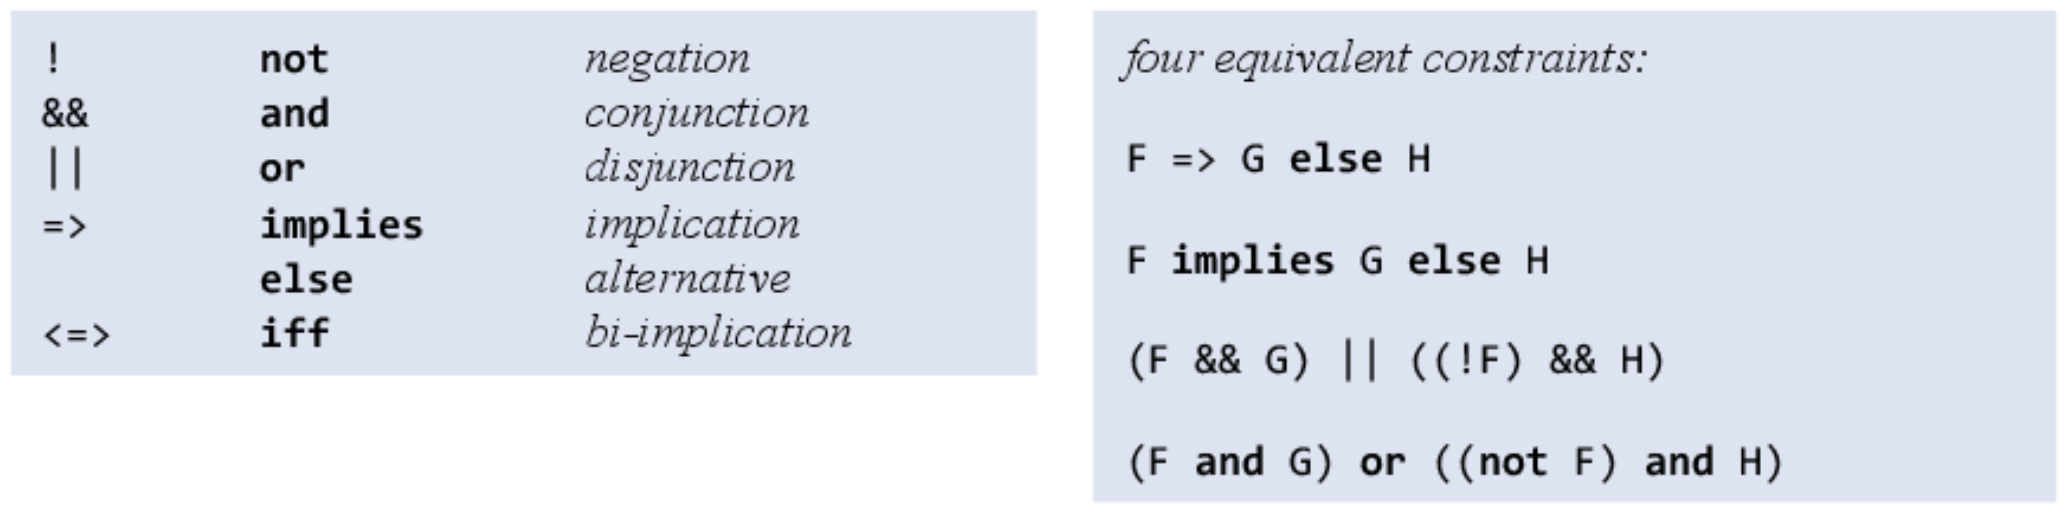
\includegraphics[width=\columnwidth]{assets/boolean}
\end{center}

\vspace{-8pt}
\textbf{Quantifiers}
\begin{center}
	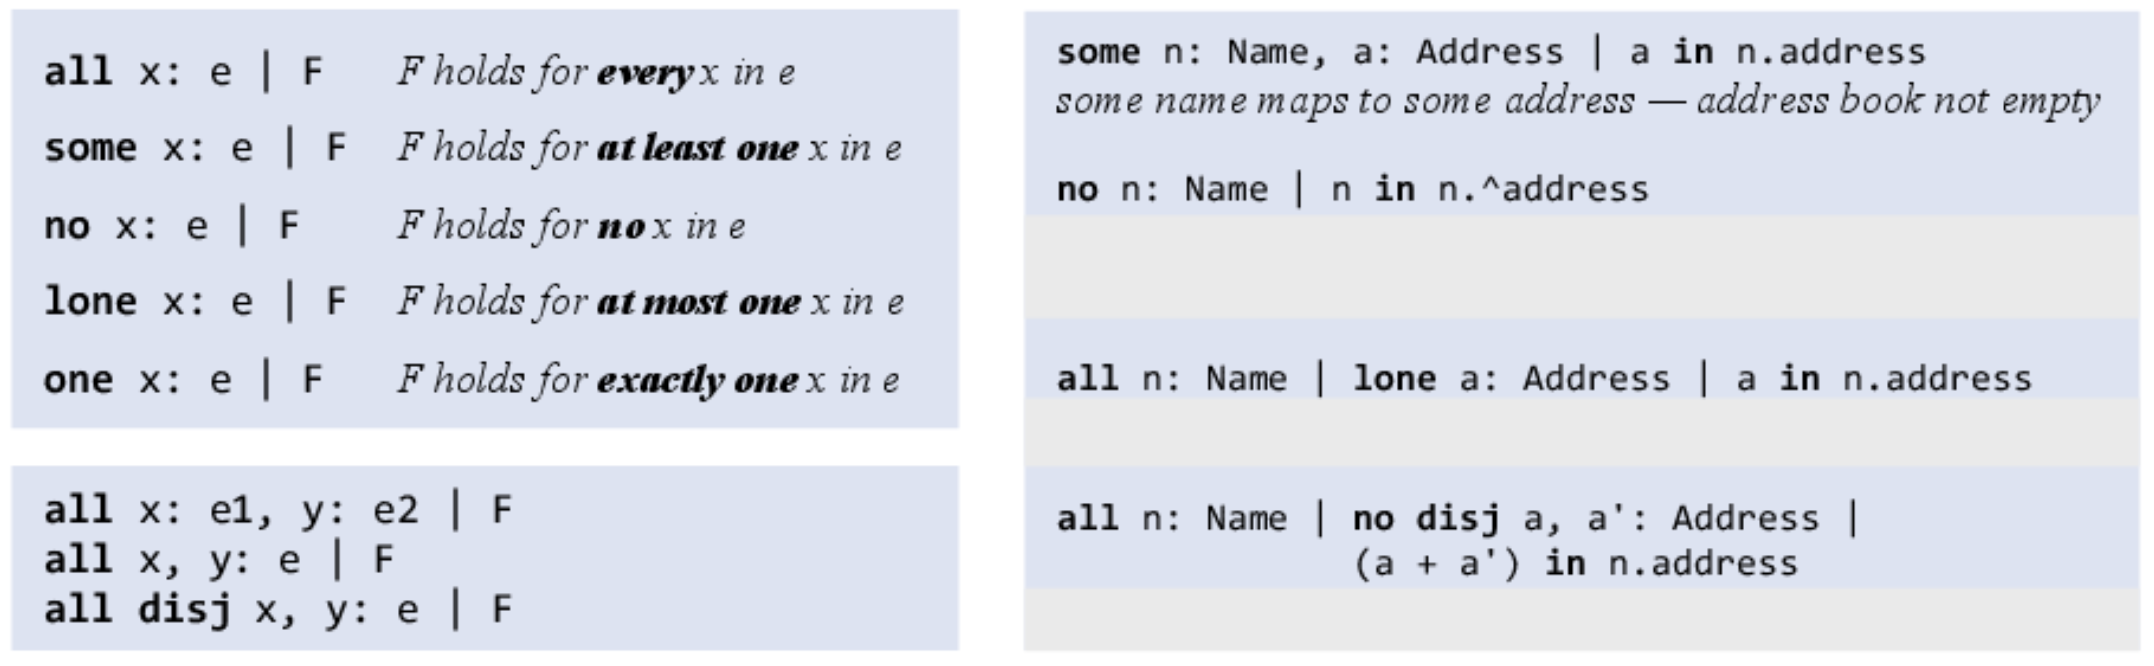
\includegraphics[width=\columnwidth]{assets/quantifiers}
\end{center}

\vspace{-4pt}
\textbf{If and Let}
\begin{center}
	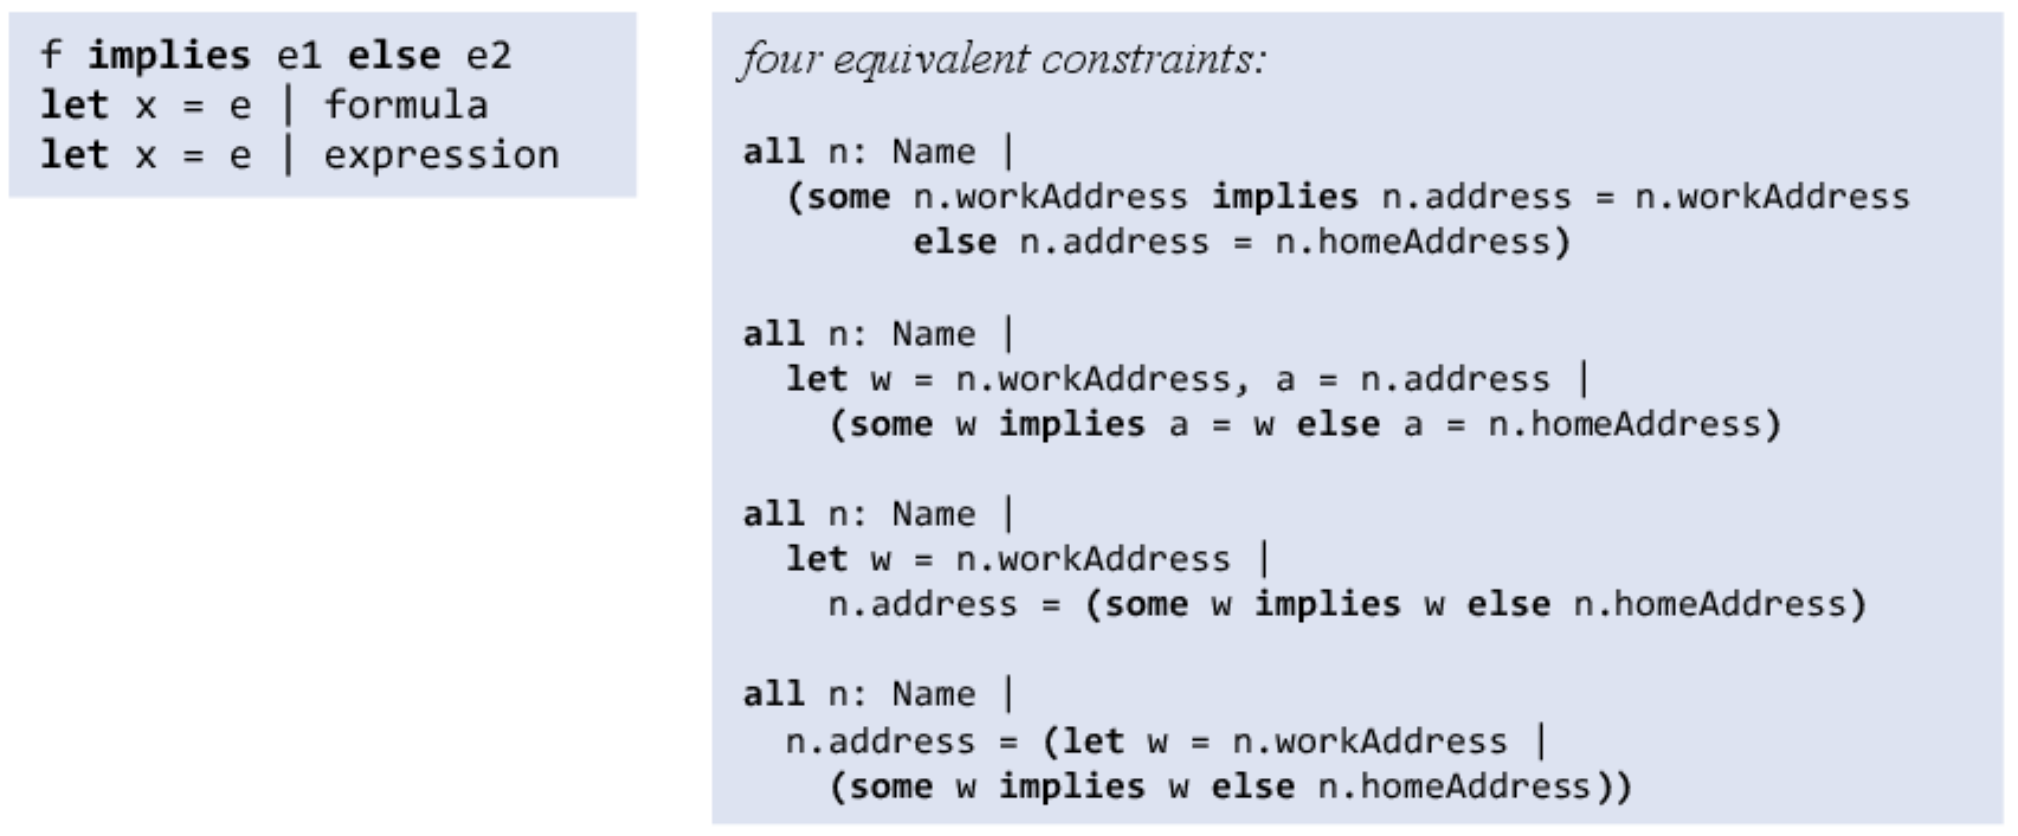
\includegraphics[width=\columnwidth]{assets/if}
\end{center}

\textbf{Cardinalities}
\begin{center}
	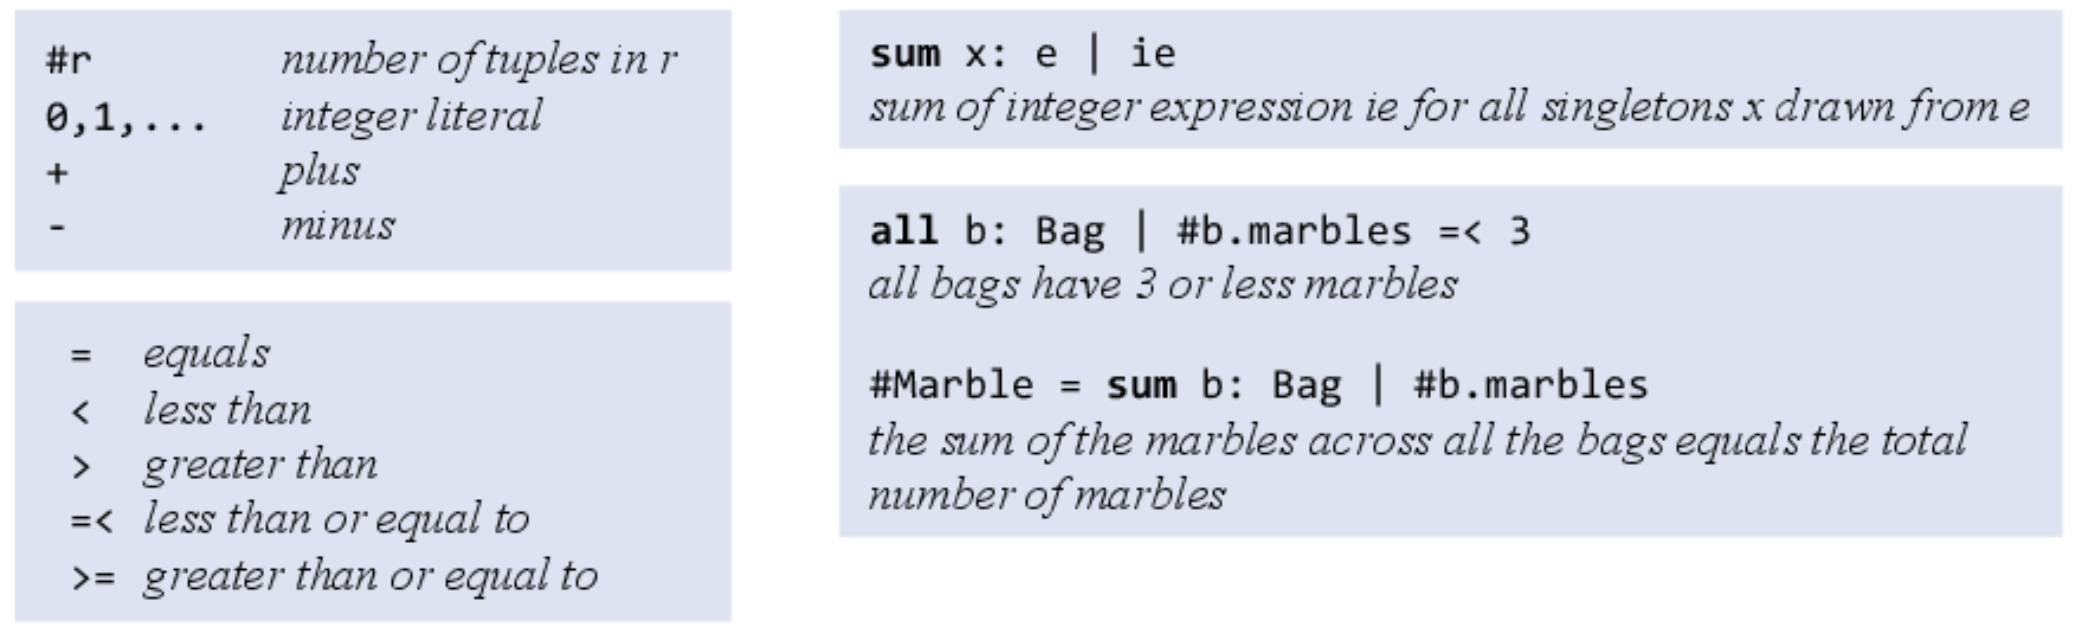
\includegraphics[width=\columnwidth]{assets/cardinalities}
\end{center}


\subsection{Static Models}

A signature declares a set of atoms (can be thought of like a class) \texttt{sig FSObject\{\}}, extends-clauses declare subset relations \texttt{sig File extends FSObject\{\}}. Like classes, signatures can be \texttt{abstract}. Further, they may constrain the cardinality of the declared set by \texttt{one, lone, some} (singleton, singleton or empty, none empty set). \\

Fields declare relations on atoms \texttt{sig A \{ f: e\}}. \texttt{f} is a binary relation on domain \texttt{A} and the range given by \texttt{e}. Range expressions may denote multiplicities \texttt{one, lone, some, set}. Fields may range over relations, with the relation declaration may including multiplicities on both sides \texttt{enrollment: Student set -> one Program}. \\

Predicates are named, parameterized formulas: \texttt{pred p[x1:e1, ..., xn:en]\{F\}}.\\

Functions are named, parameterized expressions: \texttt{fun f[x1:e1, ..., xn:en]:e \{F\}}\\

Facts add constraints that always hold, they express value and structural invariants on the model. \\

The alloy analyzer can search for structures that satisfy a constraint \texttt{C} in a model using \texttt{run C}. The existence of structures that satisfy constraints in a model is generally undecidable. The alloy analyzer searches exhaustively for structures up to a given size, therefore the problem becomes finite and decidable (e.g. \texttt{run show for 5}).\\

Exploring by manual inspection can be cumbersome. Alloy supports searching for structures that violate a given property by using \texttt{assert a \{F\}} and \texttt{check a scope}. Under-constraint models permit undesirable structures, while over-constraint models exclude desired ones.


\subsection{Dynamic Models}

Alloy 6 has a built-in notion of time based on Linear Temporal Logic (LTL). This allows us to model things like a game of ping pong. \\

LTL is boolean logic augmented with two temporal operators \texttt{next} ($X$ or $\circ$) and \texttt{until} ($U$ or $\cup$).
\begin{center}
	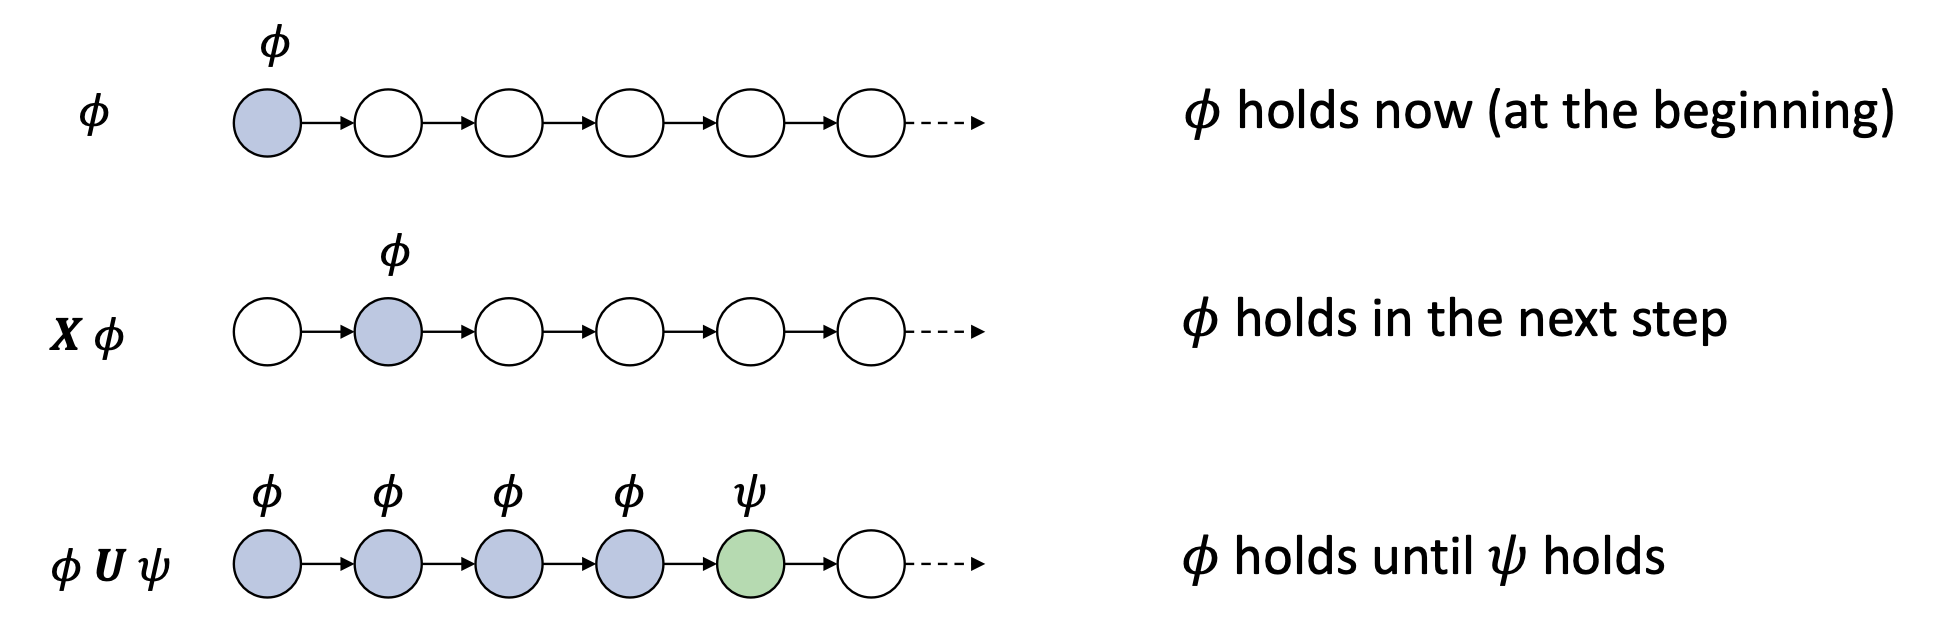
\includegraphics[width=\columnwidth]{assets/ltl}
\end{center}

From this we can derive two more operators \texttt{eventually} ($F$ or $\lozenge$) and \texttt{always} ($G$ or $\Box$). \\

Combined with mutable fields, dynamic behavior in Alloy can be summarized like this:
\begin{center}
	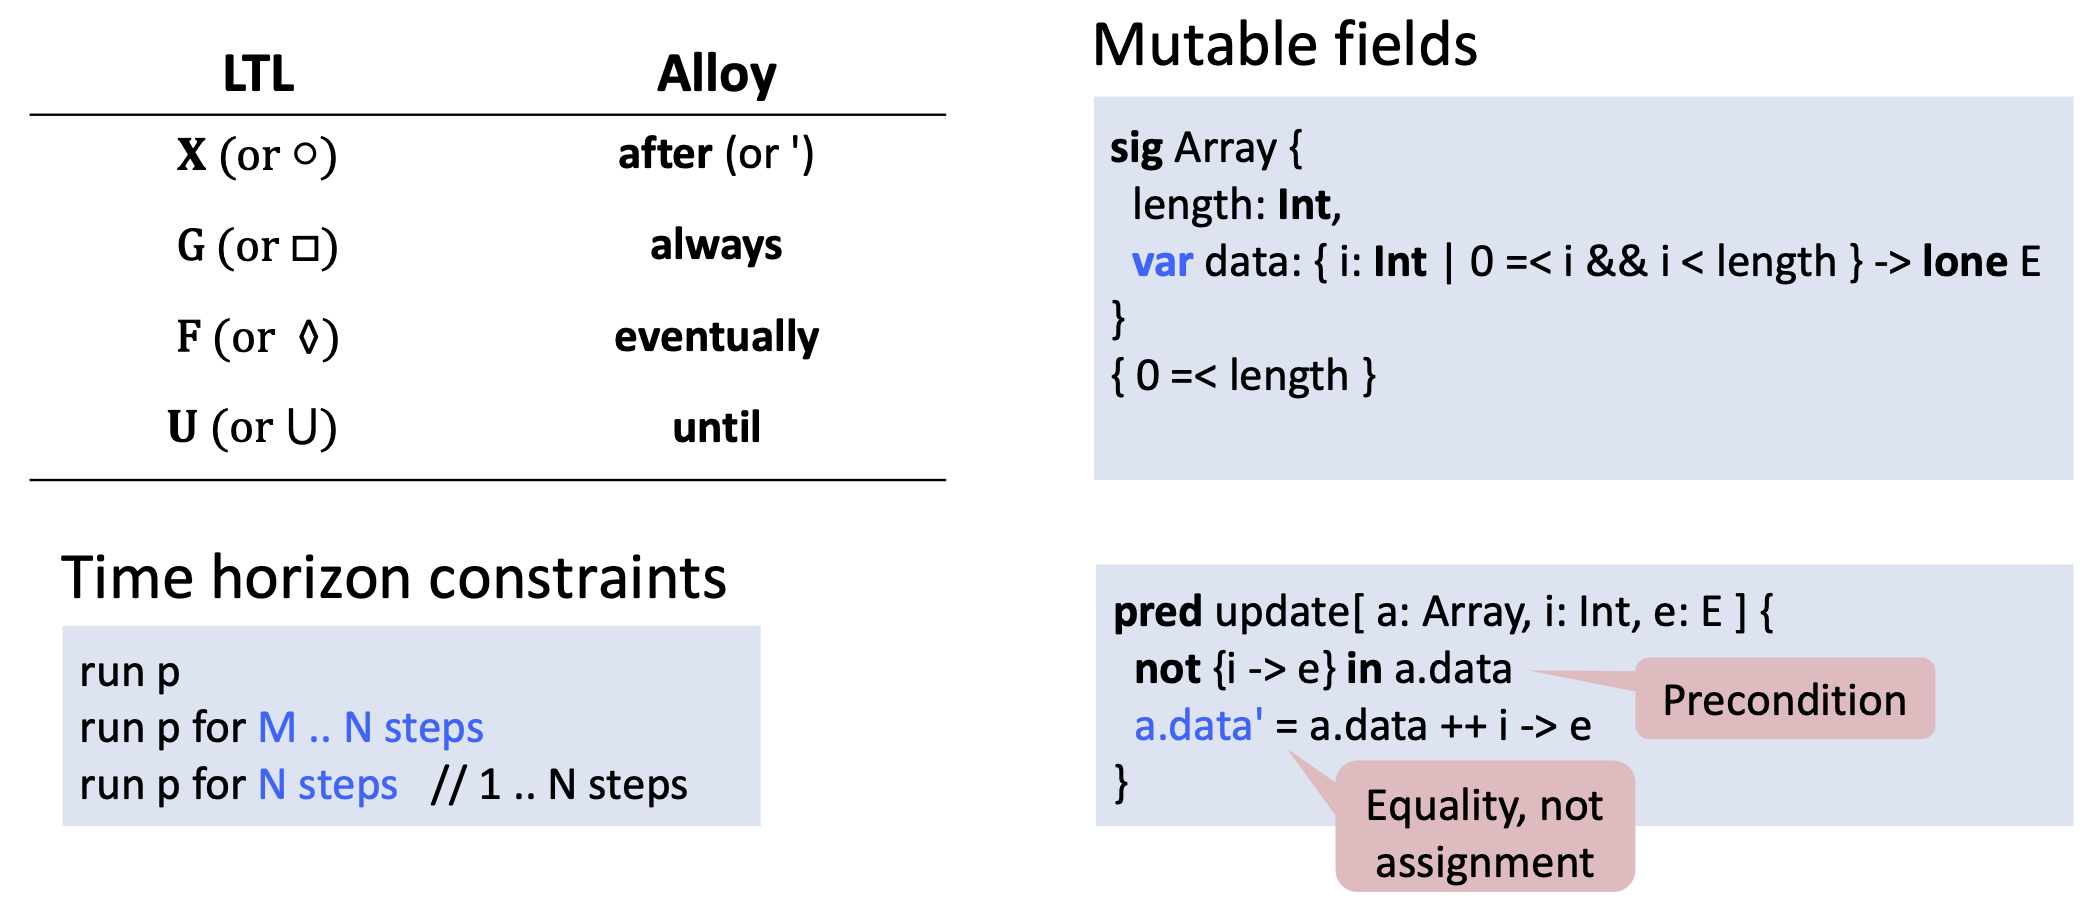
\includegraphics[width=\columnwidth]{assets/dynamic_alloy}
\end{center}

Alloy specifications are purely declarative, they describe what is done, not how it is done. Traces define the temporal behavior of the model. A first state is initialized and subsequent states are constraint using LTL operators.


\subsection{Analyzing Models}

An Alloy model specifies a collection of constraints $C$ that describe a set of structures.\\

A formula $F$ is \textbf{consistent} (satisfiable) if it evaluates to true in at leas one of these structures:
$$\exists s : C(s) \wedge F(s)$$

A formula $F$ is \textbf{valid} is it evaluates to true in all of these structures:
$$\forall s : C(s) \Rightarrow F(s)$$

Validity and consistency checking for Alloy is undecidable. The Alloy analyzer sidesteps this problem by only checking within a given scope, defining a finite bound on the size of the sets in the model. \\

In practice, SAT solvers are extremely efficient at checking consistency (performed using the \texttt{run} command). A satisfying assignment can be translated back to relations and then visualized. However, if the SAT solver returns unsatisfiable, there may exist larger structures that satisfy the conditions. \\

For validity instead of checking directly, the Alloy analyzer checks for invalidity, that is, it looks for counterexamples (performed using the \texttt{check} command).
\section{SAT/SMT-based Analysis}


\subsection{SAT Solving Algorithms}

The process of SAT solving looks as follows:
\begin{center}
	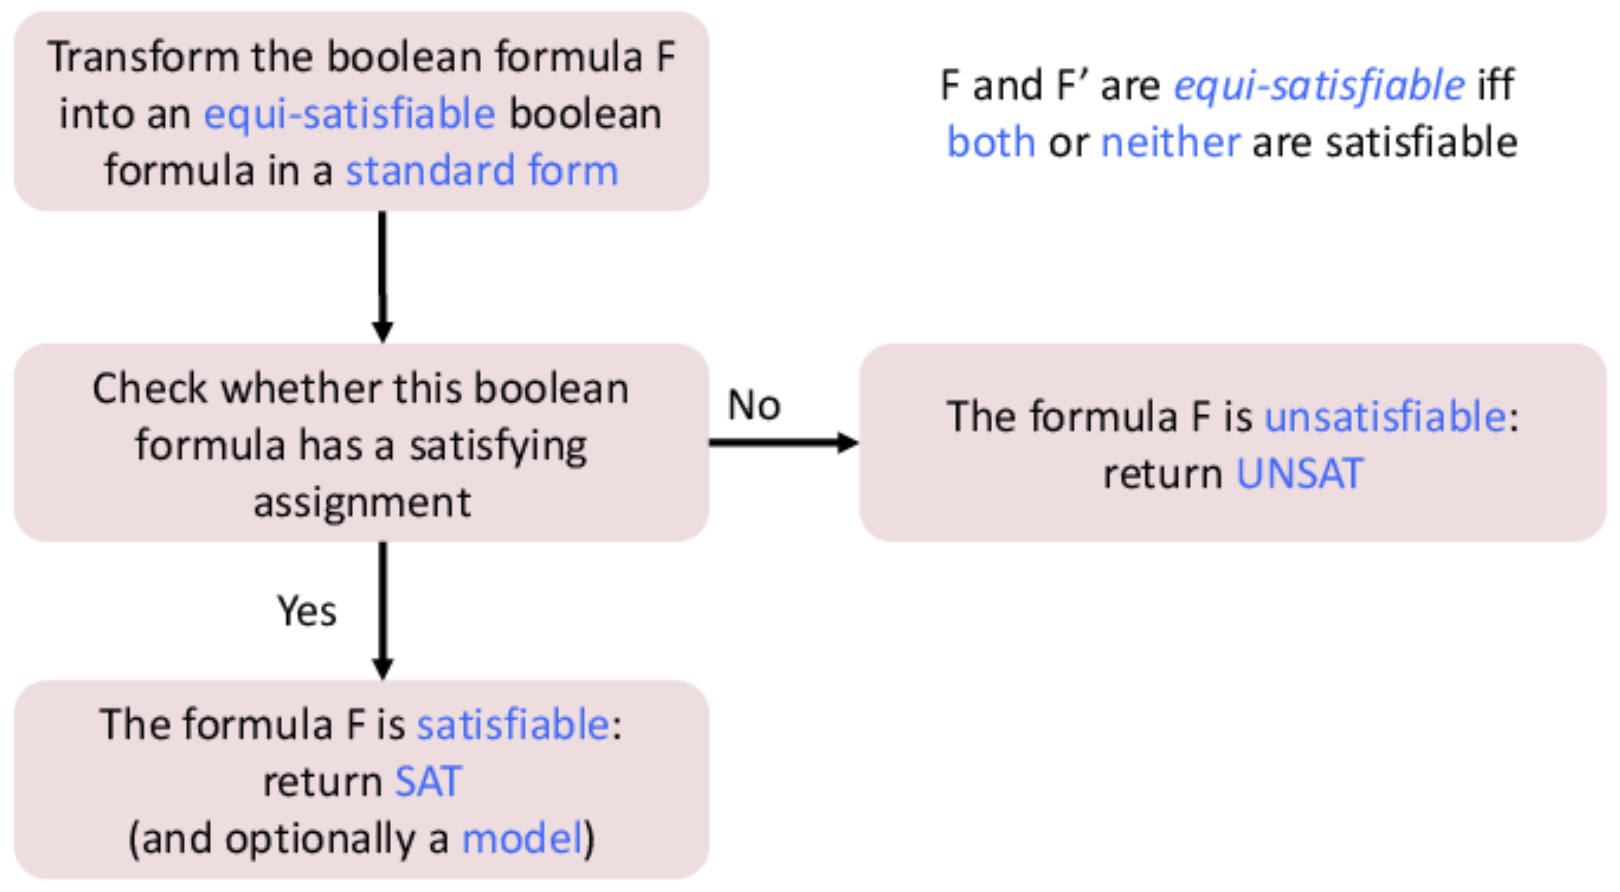
\includegraphics[width=\columnwidth]{assets/sat_solving}
\end{center}

As the standard form we use the conjunctive normal form (CNF). A formula $F$ is in CNF iff it is a conjunction of clauses. A clause is a disjunction of literals (a literal being a variable or its negation). A formula in CNF cloud look like this:
$$(p \vee \neg q) \wedge (q \vee r \vee \neg p) \wedge (s \vee p)$$

Simple conversion to CNF works as follows:
\begin{enumerate}
	\item Rewrite all $A \Rightarrow B$ to $\neg A \vee B$ and $A \Leftrightarrow B$ to $(\neg A \vee B) \wedge (A \vee \neg B)$
	\item Push all negations inwards
	\item Rewrite all $\neg \neg A$ to $A$
	\item Eliminate $\top$ and $\bot$
	\item Distribute disjunctions over conjunctions, e.g. rewrite $A \vee (B \wedge C)$ to $(A \vee B) \wedge (A \vee C)$
	\item Remove duplicate clauses and duplicate literals from clauses
\end{enumerate}

The CNF formula can be rewritten until the set is empty or a clause is empty, by using the Davis-Putman-Logemann-Loveland (DPLL) Algorithm. If the set is empty return SAT (and a model $M$, if a clause is empty return UNSAT. The rules are as follows:
\begin{itemize}
	\item Pure Literal: If $p$ occurs only positively in $F$, delete the clauses in which $p$ occurs, $M = M \cup \{p\}$ (similar if $p$ only occurs negatively.
	\item Unit propagation: If $u$ is a unit clause in $F$, delete the clauses in which $u$ occurs, update all clauses containing $\neg u$ as a disjunct by removing that disjunct, $M = M \cup \{ u \}$.
	\item Decision: If $p$ occurs both positively and negatively in F: 
	\begin{itemize}
		\item apply the algorithm to $F \wedge p, M \cup \{p\}$: if we get (SAT, $M$) then return this result
		\item otherwise, apply the algorithm to $F \wedge \neg p, M \cup \{ \neg p\}$ and return the result
	\end{itemize}
\end{itemize}


\subsection{Encoding Integers into SAT}

Alloy supports integers. Bounded integers are encoded using bit-blasting. The idea is that a 32-bit integer is a sequence of 32 individual bits. This is similar to how a circuit defines integer operations. In Alloy the bit width defines the bound for the maximum size of an integer.


\subsection{Universal Quantifiers in SMT}

When dealing with uninterpreted (user-defined) functions, the idea is to find a candidate model $M$ for the non-quantified part of the formula $F$ and check if $M$ satisfies all the universal quantifiers from $F$. This is called Model-Based Quantifier Instantiation (MBQI). In general, termination is not guaranteed when using MBQI.

\section{Modeling and Analysis of\\ Memory Models using Alloy}

Memory models are the interface between programs and their possible executions. They determine which behavior the memory and thus a program is allowed to have. In particular: from which writes can the read operations read from. A memory model would be sequential consistency or x86 Total Store Order (TSO) (a superset of sequential consistency).


\subsection{Axiomatic Semantics}

A rigorous description of the memory model. Axiomatic semantics defines events, relations, and rules. For x86 TSO we consider the following events: \texttt{read, write, fence}. \\

Program order relations $po$ orders the events in the same thread (given by program). Reads from relations $rf$ associate each read event which exactly one write. Happens before relations $hb$ guarantee that the effect of $e_1$ are visible to $e_2$. This leads us to the following axiomatic semantic rules for x86 TSO:
$$\frac{w \xrightarrow{rf} r}{w \xrightarrow{hb} r} \qquad \frac{e_1, e_2 \text{ access same variable}}{e_1 \xrightarrow{hb}�e_2 \vee e_2 \xrightarrow{hb}�e_1}$$

$$\frac{w, r, w' \text{ access same variable } w \xrightarrow{rf} r \wedge w \xrightarrow{hb} w'}{w \xrightarrow{rf} r \wedge w \xrightarrow{hb} w' \wedge r \xrightarrow{hb} w'}$$

$$\frac{e_1 \xrightarrow{po} e_2 \quad e_1, e_2 \text{ access same variable}}{e_1 \xrightarrow{hb} e_2}$$

$$\frac{e_1 \xrightarrow{po} f \quad f \text{ is a fence}}{e_1 \xrightarrow{hb} f} \quad \frac{f \xrightarrow{po} e_1 \quad f \text{ is a fence}}{f \xrightarrow{hb} e_1}$$

With these rules we can check if a given execution is allowed, by iteratively applying the rules until no new relations are added. The execution is allowed iff $hb$ is acyclic.


\subsection{Axiomatic Semantics in Alloy}

The events and axiomatic rules over the $po, rf$ and $hb$ relations can be encoded in the Alloy solver:
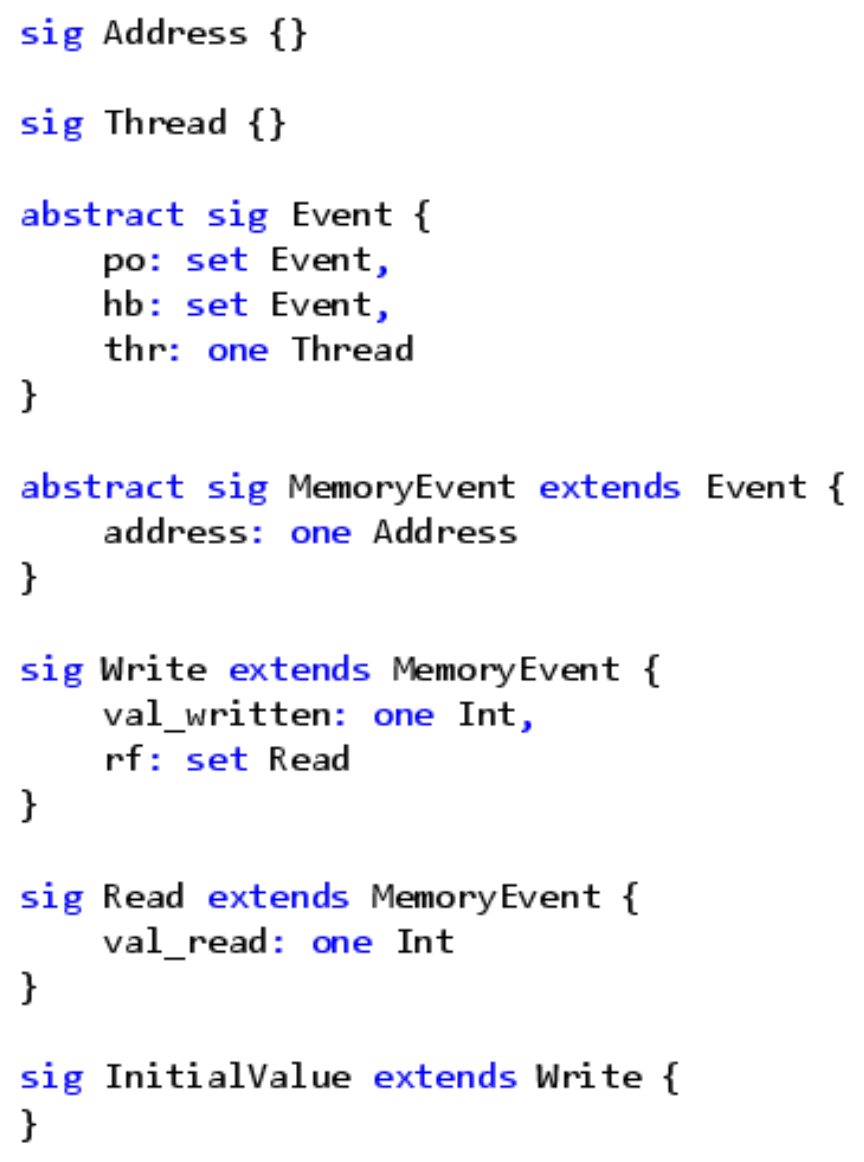
\includegraphics[width=0.6\columnwidth]{assets/axiomatic_semantics}

From there we can add all the rules as constraints.


\subsection{Memory Model Evaluation \\Framework}

Based on documentation, we can build a formal Remote Memory Access (RMA) model in Alloy. Then automatically generate tests, together with their allowed executions by the formal RMA model. After running the tests on real RMA networks we can compare the real executions with executions allowed by the model.
\begin{center}
	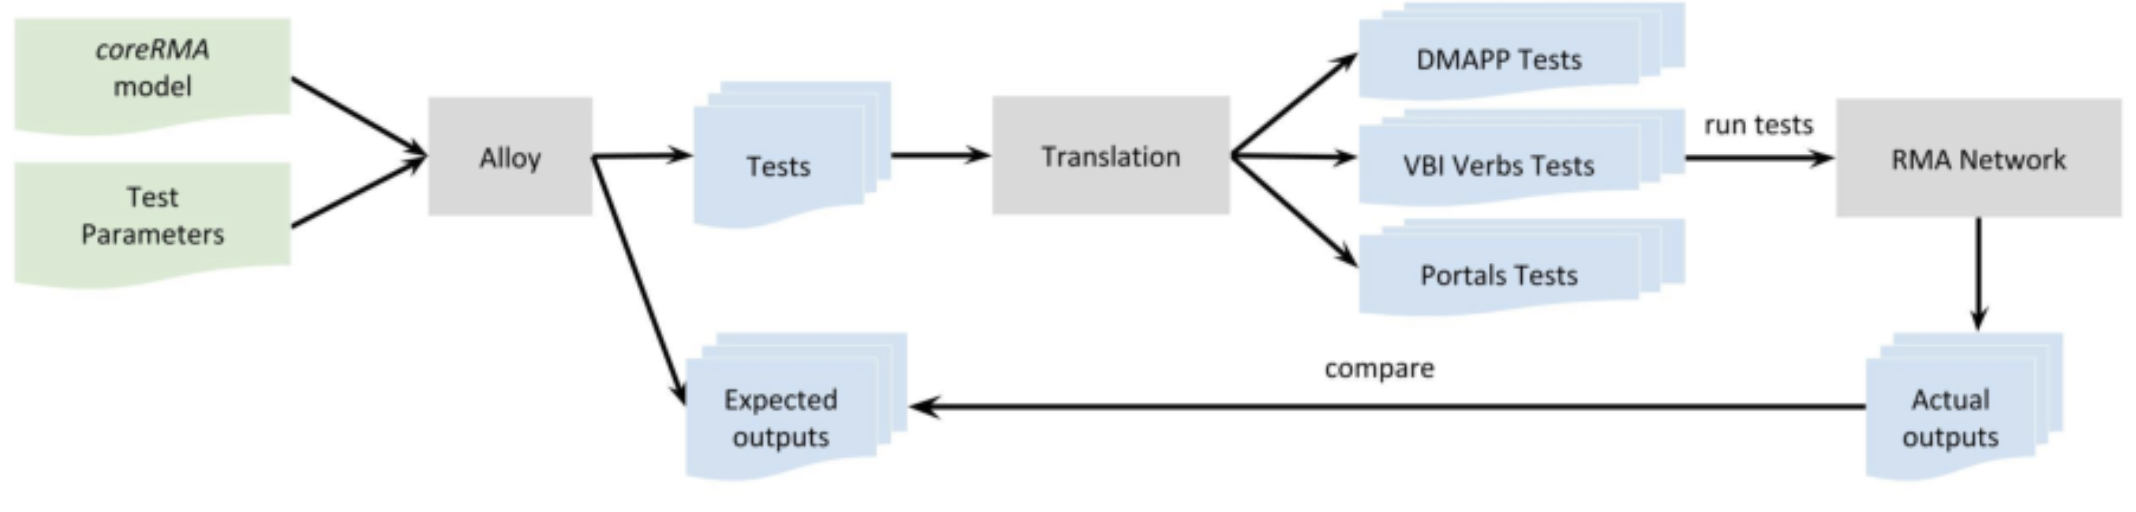
\includegraphics[width=\columnwidth]{assets/coreRMA}
\end{center}


\end{multicols*}
\end{document}

% ____ FOOTER ______________________________________________________
% Content and Template: 
% original by Danny Camenisch (dcamenisch@inf.ethz.ch), 2022
% based on different summaries from many helpful people
